\documentclass[journal]{IEEEtran}

\ifCLASSINFOpdf
   \usepackage[pdftex]{graphicx}
\else
   \usepackage[dvips]{graphicx}
\fi

\usepackage{amsmath,amssymb,amsfonts}
\usepackage{array}
\usepackage{booktabs}
\usepackage{cite}
\usepackage{graphics}
\usepackage{hyperref}
\usepackage{multicol}
\usepackage{multirow}
\usepackage{url}

\hyphenation{op-tical net-works semi-conduc-tor}

\begin{document}

\title{Multi-relational Graph Attention Networks for Real-time Traffic Prediction}

\author{
    \IEEEauthorblockN{
        Jing Huang\href{https://orcid.org/0000-0002-3294-5725}{
\includegraphics[scale=0.06]{pictures/ORCID.png}}\IEEEauthorrefmark{1},
        Kun Luo\href{https://orcid.org/0000-0002-6260-987X}{
\includegraphics[scale=0.06]{pictures/ORCID.png}}\IEEEauthorrefmark{1},
        Longbing Cao\href{https://orcid.org/0000-0003-1562-9429}{
\includegraphics[scale=0.06]{pictures/ORCID.png}}, \textit{Senior Member}, \textit{IEEE}\IEEEauthorrefmark{2},
        Yuanqiao Wen\IEEEauthorrefmark{3},
        Shuyuan Zhong\IEEEauthorrefmark{1}}
    \thanks{Manuscript received xxx; revised xxx; accepted xxx.}
    \thanks{This work was supported by the National Natural Science Foundation of China (No. 52072287) and Zhejiang  Provincial  Science  and  Technology  Program (No. 2021C01010)}
    \thanks{Jing Huang, Kun Luo and Shuyuan Zhong are with the School of Computer Science and Artificial Intelligence, Wuhan University of Technology, Wuhan 430063, China (Corresponding auther: Jing Huang, e-mail: huangjing@whut.edu.cn).}
    \thanks{Longbing Cao, IEEE Senior Member, is with the Advanced Analytics Institute, University of Technology Sydney, Sydney, NSW 2007, Australia.}
    \thanks{Yuanqiao Wen is with the National Engineering Research Center for Water Transport Safety, Wuhan University of Technology, Wuhan 430063, China.}
}

\markboth{IEEE TRANSACTIONS ON INTELLIGENT TRANSPORTATION SYSTEMS}{Multi-relational Graph Attention Networks for Traffic Signal Coupling Learning and Prediction}

\IEEEtitleabstractindextext{
    \begin{abstract}
    Accurate real-time traffic prediction is of great importance to ITS, yet it remains challenging due to the complex spatio-temporal dynamics of traffic systems. The continuous traffic signals from different channels and nodes in a traffic network are coupled with each other, including temporally over time points of each signal channel, spatially between traffic nodes, and in a spatio-temporal joint manner. These multi-aspect traffic signal couplings jointly reflect the conditions of a traffic system and evolve over traffic movement and system dynamics. The recent studies have made great achievements on formulating traffic prediction as a high-profile graph neural network-based modeling problem. However, they mainly focus on several well-known hidden relations captured by neural graph mechanisms while the exploration on the above multi-aspect interactions coupling diverse traffic signals are quite limited. This work views a traffic system as a \textit{coupled traffic network} and models the \textit{multi-aspect traffic signal couplings} by a Multi-relational Synchronous Graph Attention Network (MS-GAT). Specifically, the proposed MS-GAT learns three separate embeddings to respectively represent the traffic signal-based channel, temporal and spatial relations between nodes in a synchronous manner through specific graph attention networks, which are further adaptively coupled according to their respective importance to predictions. Tested on five real-world datasets, MS-GAT proves to outperform six state-of-the-art graph network-based traffic predictors, showing its value on capturing not only spatial and temporal relations over coupled traffic signals, but also the traffic signals-based channel relations and their couplings over the traffic evolution.
    \end{abstract}
    \begin{IEEEkeywords}
        Traffic prediction, multi-relational modeling, spatio-temporal graph modeling, graph attention networks, coupled traffic network, coupling learning, traffic signal coupling.
    \end{IEEEkeywords}
}

\maketitle

\IEEEdisplaynontitleabstractindextext
\IEEEpeerreviewmaketitle

\section{Introduction}
\label{sec:introduction}

\IEEEPARstart{D}{ata}-driven traffic prediction  \cite{vlahogianni2014short} is a critical task of intelligent transport systems (ITS). It is of great value for various real-world applications such as efficient traffic management, dynamic route planning, and intelligent guidance service. Traffic prediction estimates the future traffic conditions based on historical observations of traffic systems such as physical road networks. Traffic conditions are reflected on temporal and spatial traffic signals such as channel or node-based traffic volume, density, speed, and others captured by diverse sensors deployed at different geospatial locations in a traffic network. All aspects of traffic signals are coupled with each other temporally and spatially, forming a \textit{coupled traffic network}, similar to many other complex systems where objects and their attributes interact and couple with each other \cite{2015Coupling,WangGC21}. For example, the traffic conditions at one traffic node may be associated with those at its neighbouring and farther nodes before and after along the traffic network, forming \textit{spatial relations} between traffic network nodes. Second, the traffic signals of one node may be temporally related to those of backward and forward nodes, forming \textit{temporal relations}. Both spatial and temporal relations are node- and time-evolving, the same as the traffic conditions. They are further subject to the burst of traffic accidents and special events taking place on the road. Moreover, the spatial and temporal relations are interdependent, forming \textit{spatio-temporal relations} in traffic systems. In addition, similar to the user-item interations in recommender systems \cite{cao2016non}, the spatio-temporal interactions in a traffic network and among its traffic conditions may be explicit and implicit, and hierarchical and heterogeneous \cite{zhu2020unsupervised}. These multi-aspect interactions and couplings make it difficult to precisely predict how the rise of vehicle flow at one node at a time point may cause the change of vehicle flows at other nodes at future time steps. It is thus essential yet challenging to effectively model the various spatio-temporal traffic signal couplings over channels and nodes, which could better capture the intrinsic characteristics and complexities in traffic networks, leading to better traffic modeling and prediction.

Extensive data-driven methods have been employed to analyze some relations in traffic systems in a road network, which can be categorized into time-series methods, shallow machine learning methods, and deep learning methods. First, at the early stage, traditional time-series methods such as  historical average model \cite{liu2004summary}, auto regressive integrated moving average (ARIMA) \cite{williams2003modeling}, Kalman filtering model \cite{OKUTANI19841} and canonical  vector auto regressions (VAR) \cite{zivot2006vector} were widely used in traffic forecasting. Then, shallow machine learners such as Support Vector Regression (SVR) \cite{1364002}, Bayesian model \cite{1603558} and $k-$nearest neighbor method \cite{zhang2009short} have been developed. Recently, deep neural networks (DNNs) has dominated the research on traffic prediction by capturing sequential relations in a large amount of traffic sequential data \cite{lv2014traffic}, \cite{yu2017deep}. For example, temporal dependencies are modeled in \cite{zhao2017lstm} and \cite{ma2015long} by recurrent neural networks (RNNs). In \cite{wu2016short,ma2017learning,zhang2017deep}, spatial dependencies are captured by convolutional neural networks (CNNs). However, both RNNs and CNNs are insufficient in modeling spatio-temporal traffic interactions. Fortunately, they are more successfully characterized by the recent advances in graph neural networks (GNNs). GNNs present the interactions between entities as a graph and can capture spatial node interactions in a road network \cite{wu2020comprehensive, jiang2021graph}. Recent methods based on GNNs including STGCN \cite{yu2017spatio}, DCRNN \cite{li2017diffusion}, Graph WaveNet \cite{wu2019graph} and AGCRN \cite{bai2020adaptive} formulate the traffic prediction as a spatio-temporal graph modeling problem and have achieved superior performance in traffic forecasting. GNN-based models focus on optimizing the representation of either spatial relations (e.g., \cite{yu2017spatio} in urban roads by graph convolutional networks (GCN) and in \cite{li2017diffusion} based on diffusion convolutional networks) or temporal relations (e.g., learning temporal patterns in \cite{bai2020adaptive} and \cite{wang2020traffic} by gated recurrent units (GRU)).

Though DNNs including GNNs achieve the state-of-the-art traffic prediction performance by applying increasingly advanced network architectures and learning mechanisms and overparametering the networks, the current research focus is mainly on characterizing latent features and relations in a traffic network, e.g., the above spatial, temporal, and spatio-temporal features or relations. By taking a coupled traffic network view with multi-aspect traffic signals coupled, there are still various issues and data complexities that have not yet been explored or insufficiently characterized. For example, sensors deployed at a node capture various aspects of traffic signals such as speed, volume and density, which are coupled in reality and thus their relations should be jointly represented to capture the multi-view node conditions. What's more, the traffic conditions at one node or on one road may be related to that at other nodes or roads, i.e., a signal at a node and time point is essentially embedded in the entire traffic system and its dynamics. This coupled traffic network view focuses on modeling rich signal couplings and interactions in traffic systems, capable of addressing problems such that how an accident at one point may not only cause problems to its node and neighboring nodes and roads but also to other places affecting the evolving traffic network.

Specifically, based on the stronger capability of GNNs and addressing the significant gaps in modeling complex traffic systems, this work models the above multiple aspects of signal couplings and their evolution explicitly or implicitly embedded in complex traffic networks. We introduce a framework of modeling spatio-temporal traffic signal couplings (see Fig.~\ref{fig:core}), followed by a spatio-temporal graph network (see Fig.~\ref{fig:framework}), named Multi-relational Synchronous Graph Attention Networks (MS-GAT). In MS-GAT, similar to the concept of image channel in computer vision, each traffic signal is viewed as a measurement channel at a traffic node. Here, the temporal signal movement over time forms the temporal channel representation; each node is often characterized by signals collected from multiple sensors deployed on the spot, with the signals interacting with each other to capture the multi-channel interdependencies; nodes in the traffic network are further connected to capture their spatial relations. Consequently, MS-GAT captures temporal relations in each signal over time, spatial relations over nodes, and multi-channel relations between signals. These are jointly modeled for traffic prediction. By viewing traffic systems as coupled traffic networks with coupled traffic signals over sensors, our contributions are as follows:

i) We recognize the significance of a kind of latent relation (called \textit{channel relation} in this paper) and characterize this noteworthy relation in our proposed spatial-temporal graph model. To the best of our knowledge, this is the first work that explicitly models this channel relation in traffic prediction task.

ii) We propose a spatial-temporal graph model based on multi-component fusion, called MS-GAT, which is accompanied by a flexible and effective data augmentation scheme for its supervised learning process. In this model, the newly-attended channel relation together with the other two familiar relations are picked abreast up by a core module called multi-relational embedding abreast module (MEAM). Furthermore, their contributions to the resulted traffic conditions in real-world forecasting scenarios are adaptively distinguished in a synchronous manner by a developed deep framework based on our devised multi-dimensional self-attention scheme.

iii) We develop a simple yet effective multi-dimensional self-attention scheme to improve the conveniences of applying and implementing the self-attention mechanism for handling multi-dimensional input data. The scheme is also effective in ameliorating the influence of attention mechanism on model size while ensuring the prediction capability.

We conducted a series of experiments on five real-world traffic datasets. Experimental results demonstrate the superior performance of the proposed MS-GAT\footnote{The source code is publicly available from \url{https://github.com/luokn/ms-gat}}.
The remainder of this paper is organized as follows. Section II reviews the related work. The problem statement is presented in Section III. Section IV details the proposed approach. Section V reports the experimental results, followed by the discussion in Section VI. Section VII concludes the paper.

\section{Related Work}
\label{sec:related_work}
In this section, we review three sets of related work: data-driven methods, coupling learning and attention-based relation modeling, and multi-component fusion for traffic prediction.

\subsection{Data-driven traffic prediction}
Compared to knowledge-driven methods using queuing theory such as in \cite{cascetta2013transportation}, data-driven methods have dominated the recent traffic forecasting research, benefiting from the convenient acquisition of a huge amount of traffic data and the vigorous development of machine learning models. The early work on data-driven traffic forecasting mostly focuses on time series analysis, such as ARIMA \cite{williams2003modeling} and VAR \cite{zivot2006vector}, which typically rely on the stationarity assumption. To eliminate this assumption, recent research shifts to deep-learning-based models. Various efforts, e.g., \cite{zhao2017lstm,ma2015long,bai2020adaptive,pan2020spatio}, applied RNN and its variants such as LSTM \cite{hochreiter1997long} and GRU \cite{cho2014learning} to learn relations in traffic data automatically, taking advantage of the RNN’s superior ability in modeling the temporal dynamics in time series data \cite{connor1994recurrent}. However, they overlook other relations such as the spatial relations. Accordingly, other attempts based on deep learning for traffic forecasting (e.g., \cite{wu2016short,ma2017learning,zhang2017deep}) deployed CNN to pay more attention to spatial relations among the traffic series from different traffic nodes. However, due to the fact that CNN is preferable to manipulating regular grid data (e.g., 2D images), those CNN methods force the spatial structure among different traffic series into a Euclidean space which is naturally violated by real-world traffic data. Considering the structural characteristics of traffic data, more recent work leverages the GNN (e.g., GCN \cite{kipf2016semi}, a special kind of CNN generalized for graph-structured data) to model the spatial relations in traffic road networks. For example, STGCN \cite{yu2017spatio} formulates the traffic prediction problem as graphs instead of applying regular recurrent and convolutional neural units in a deep learning architecture. In the same manner, DCRNN \cite{li2017diffusion}, Graph WaveNet \cite{wu2019graph} and GSTNet \cite{fang2019gstnet} utilized various GCNs to capture the prominent spatial interactions among different traffic series. Their efforts gain the state-of-the-art performance, thus opening a new door for traffic prediction. In contrast, our work in this paper is also based on GCN (\cite{mengzhang2020spatial, song2020spatial}) to model a traffic system as a spatio-temporal graph. We pay attention not only to the different relations embedded in a graph structure but also to their coupling strengths with each other. Our method innovatively models the traffic signals-based channel relations indispensable and hidden in a dynamic evolving systems like road  networks. This channel relation modeling complements with the spatio-temporal prediction for capturing more comprehensive traffic conditions. Note that the traffic data we discuss in this paper refers to the readings of traffic signals acquired by a variety of geo-sensors in a traffic road network, e.g., traffic flow or speed. 

\subsection{Coupling learning and attention-based relation modeling}
Complex systems like traffic networks are embedded with hierarchical and heterogneous coupling relationships and interactions within and between entities, subsystems and systems. Coupling learning captures the relationships and interactions in various settings, \cite{Huaaai19,2018CoupledCF}. They involve various techniques including incorporating metric learning, representation learning, multikernel learning, coupled hidden markov models and deep neural networks into modeling complex couplings and interactions\footnote{Interested readers may find more in https://datasciences.org/coupling-learning/.}. This paper expands coupling learning to learn multi-aspect traffic signal couplings by treating a traffic system as a coupled traffic network.

The attention mechanism is initially used in neural machine translation tasks \cite{bahdanau2014neural}. Its core idea is to adaptively pick up features that are relatively critical to specific tasks by learning the relations hidden inside input data. In recent years, it has been widely applied in various sequence-to-sequence (seq2seq) issues, such as air quality forecasting \cite{cheng2018neural} and sequential recommendation \cite{2018CoupledCF}. Typically, self-attention \cite{vaswani2017attention, velivckovic2017graph}  has been applied in traffic prediction to  model dependencies, as shown in traffic prediction models like GeoMAN \cite{liang2018geoman} using a multi-level attention-based recurrent neural network to predict the readings of a geo-sensor over several future hours and ASTGCN \cite{guo2019attention} implementing an attention-based spatial-temporal graph convolutional network for traffic flow forecasting. GMAN \cite{zheng2020gman} proposes a graph multi-attention network in an encoder-decoder architecture to carry out long-term traffic prediction. All the attention-based prediction models (e.g., \cite{liang2018geoman, guo2019attention, zheng2020gman, cai2020traffic, fang2020constgat, park2020st, chen2020multi}) tend to improve the effect of capturing spatio-temporal dependencies by leveraging self-attention to cooperate with the related convolutional operations. However, considering that the input and output of a self-attention module are generally two sequences of vectors, existing prediction models either develop self-attention separately in the spatial dimension of traffic conditions or in its temporal dimension, and thus they can not be easily deployed in a multi-dimensional information space. Even if their self-attention processes are stubbornly implemented on each dimension of multi-dimensional input data in turn, the resultant model will fall into such dilemmas of a large parameter scale and the code-level redundancy. To this end, we aim to synchronously capture several sorts of significant relations among multi-dimensional traffic data. Thus, a multi-dimensional self-attention scheme is proposed to universally and conveniently model different information dimensions of input data with less computational and development costs.

\begin{figure*}[!ht]
    \centering
    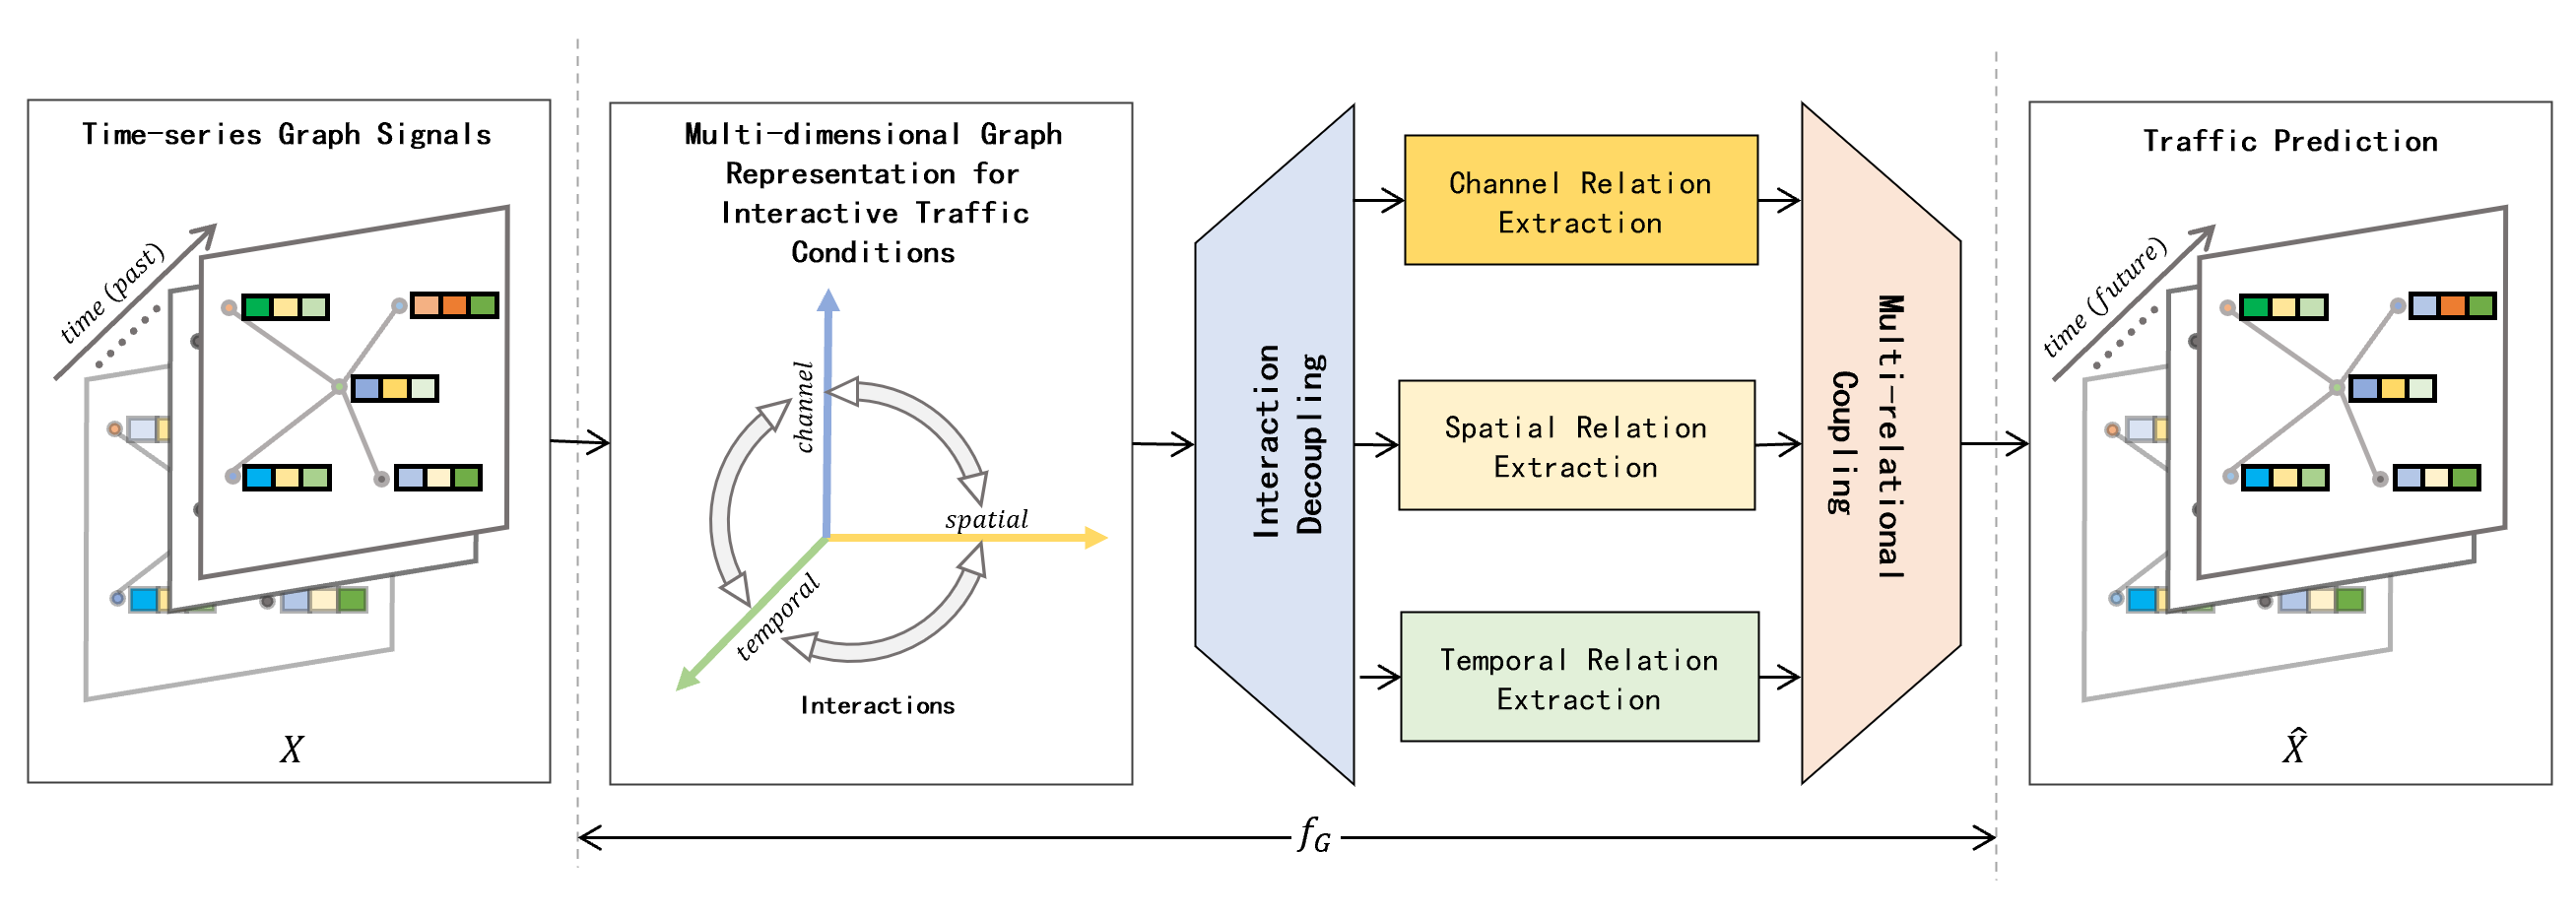
\includegraphics[width=0.9\textwidth]{pictures/Core.png}
    \caption{The framework of modeling spatio-temporal traffic signal coupling relationships from multiple channels in a dynamic traffic system. It forms a three-dimensional graph representation of interactive traffic conditions and further provides a multi-relational view of traffic prediction, where the temporal, spatial and channel relations are explicitly and implicitly coupled in the entire evolving traffic network. Our method firstly decouples them for separate representations and then couples their representations to formulate a multi-relational traffic graph.}
    \label{fig:core}
\end{figure*}


\subsection{Multi-component fusion}
The idea of multi-component fusion originates from ensemble learning \cite{dong2020survey}. In ITS, a few studies have leveraged the multi-component architectural style to deploy specific learning models for various tasks. For instance, \cite{geng2019spatiotemporal} shows a novel deep learning model  ST-MGCN for ride-hailing demand forecasting. For forecasting traffic flow in a road network, ASTGCN \cite{guo2019attention} enjoys a great success by adopting a gated mechanism based on time embedding to fuse multiple components. In contrast, our method MS-GAT also involves the multi-component fusion by using a time-gated mechanism for traffic prediction, it is more flexible in the preparation of training samples, which is crucial to the final performance and generalization capability of a supervised learning model. Specifically, instead of fixing the input sequence of each component by intuitively judging the importance of the chosen input sequence (e.g., \cite{guo2019attention}), our multi-component fusion design can provide richer and more diverse time-series graph data for the supervised learning according to the genuine importance of the input time-series graph data of each component to the same output sequence. In other words, our design is equipped with an effective data augmentation scheme, which can make full use of all the observed data along the time-axis to pick up their latent patterns sensitive to prediction.


\section{Problem Statement}
\label{sec:problem_statement}

The road network of a transport system is characterized as a directed graph $G = (V, E, A)$, where a set of $N = |V|$ vertices $V$ denote the traffic nodes (e.g., sensors deployed in the traffic network); a set of edges $E$ depict the connectivity among nodes; and the adjacency matrix $A \in \mathbb{R}^{N \times N}$ describes the connectivity in the network, where $A_{u,v}=1$ refers to a connection between node $u$ and node $v$, otherwise zero.

\begin{figure*}[!ht]
    \centering
    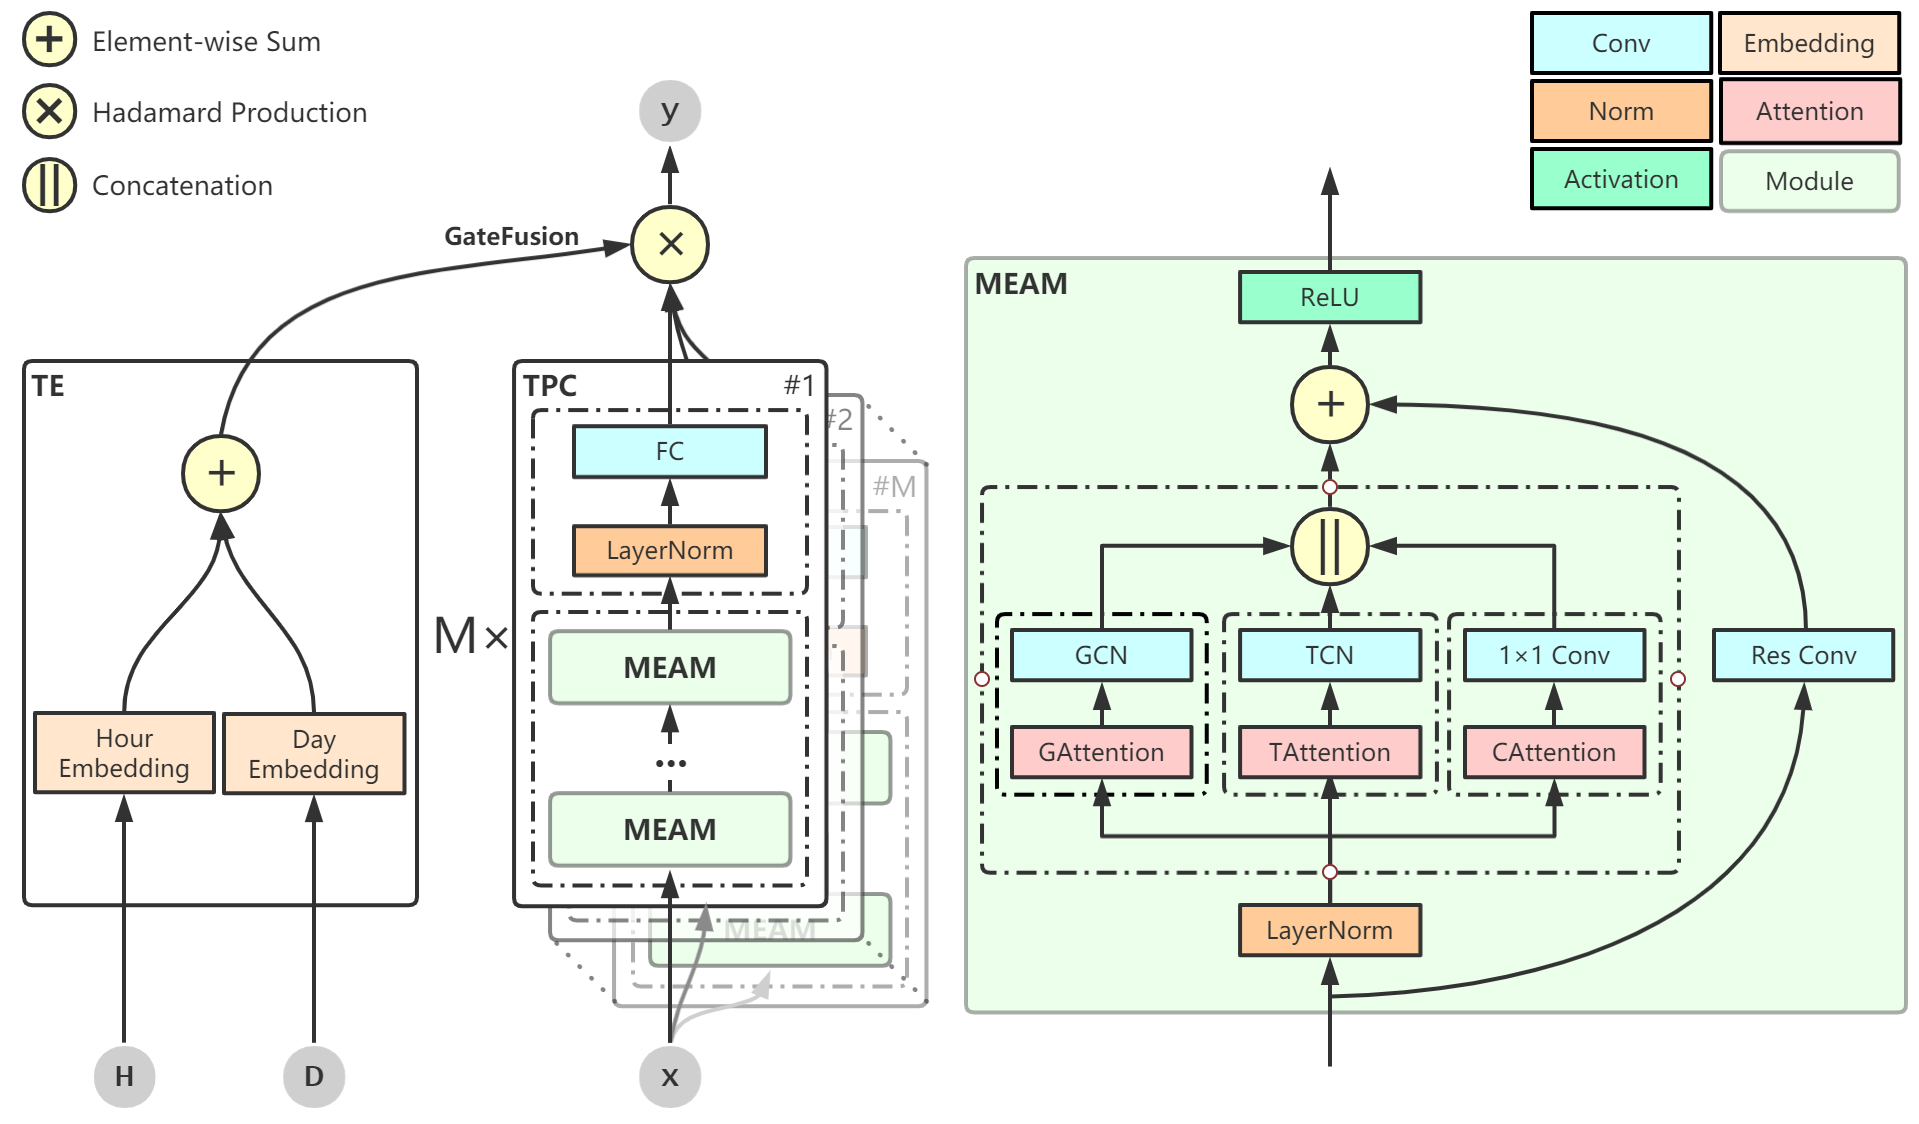
\includegraphics[width=0.64\textwidth]{pictures/Framework.png}
    \caption{An overview of the proposed MS-GAT to model multi-aspect traffic signal couplings. Left: Architecture of MS-GAT, which adopts the multi-component structure with time-gated fusion. Right: Core module of MS-GAT, i.e., multi-relational embedding abreast module (MEAM), which implements the interaction decoupling and multi-relational couplings respectively at its two ends by our multi-dimensional attention mechanism, while learning the embeddings of spatial relations, temporal relations and channel relations in a synchronously handling manner.}
    \label{fig:framework}
\end{figure*}

In a traffic network, all traffic conditions $X$ describe the status of the network. Traffic conditions are multivariate, capturing various traffic signals such as traffic volume, density and speed. Suppose there are $d_c$ types of available traffic signals (or indicators), each traffic signal is treated as a separate information channel of traffic nodes, similar to the concept of image channel in computer vision. We then have $X=\left < X(1),\dots,X(d_c) \right >$, where each term $X(l)$ (here, $1 \leq l \leq d_c$) is a random variable to depict a traffic condition, e.g., the observations (or measurement) of traffic flow. The multivariate observations at each traffic node capture the all-channel information of that node, which is called a node’s \textit{channel dimension}. The graph corresponding to the entire traffic network is represented by the interactions between all random variables (from $X(1)$ to $X(d_c)$), which is called the \textit{channel relation} over all $d_c$ channels in the network. 
In a road network, the traffic conditions may change over time, forming a dynamic graph. Assume there are $t_p$ time steps, the traffic conditions $X$ are composed of a sequence of $t_p$ temporal random graph snapshots (each graph snapshot $X^{t}$ corresponds to the traffic network profile at a time point $t$), i.e., $X = [X^{t_1}, \dots , X^{t_p}]$. This time series describe the traffic conditions in terms of a \textit{temporal dimension} of traffic nodes, and the interdependence between time-specific traffic conditions (i.e., different graph snapshots $X^t$ and $X^{t^{'}}$, here $t_1 \leq t, t^{'} \leq t_p$) along the temporal dimension forms the \textit{temporal correlation}  in the network. 
Further, each node of the network is affiliated with multiple channels of signals, and each signal is temporal. Hence, the overall traffic conditions $X$ can also be viewed as a set of $N$ node-oriented random variables, i.e., $X = \left\{X_1, \dots , X_N\right\}$, where each variable $X_v$ denotes the traffic conditions of the node $v$, forming the \textit{spatial dimension} of a node. The interdependence between node-specific variables captures the \textit{spatial correlation} between nodes in the network.  

Accordingly, we can model a traffic network in terms of channel, temporal and spatial dimensions, which offers a three-dimensional view of a traffic system. Further, any node $v$ can be modeled by a three-dimensional vector $X_v^{t}(l)$ with its $l^{th}$ signal at time point $t$. The three dimensions further capture various traffic conditions (signals), which directly reflect the observations and characteristics of the physical traffic world. In addition, the joint modeling of their temporal, spatial and spatio-temporal relations provide a deep quantification of a complex traffic network. 

Consequently, the GNN representation of a traffic network maps a physical system with various traffic signals to a graph $G$ with nodes $\left\{X_v^{t}(l)\right\}$ over $t_p$ time steps. The problem of this GNN-based traffic prediction is to learn a mapping network $f_G$ between the $t_p$ steps of historical traffic conditions $X = [X^1,\dots, X^{t_p}]$ and the next $t_q$ steps of traffic conditions $\hat{X} = [X^{t_p + 1},\dots, X^{t_p + t_q}]$ in the graph $G$.

\begin{equation}
    [X^{t_p + 1}, \dots , X^{t_p + t_q}] = f_G(X^1, \dots, X^{t_p};\theta)
    \label{eqn:target_function}
\end{equation}

where $\theta$ stands for the learnable parameters of graph $G$.

\textbf{Our insight.} The above problem statement formulates a traffic system as a coupled traffic network where diverse traffic signales (e.g., from multiple sensors) are coupled with each, which differs from the existing assumptions and methods. Figure~\ref{fig:core} illustrates the framework of modeling spatio-temporal traffic signal couplings in a dynamic coupled traffic network with various channels and nodes by a multi-relational graph. Our model extracts the channels of traffic signals, temporal signal development, and interactions between signals at each node, between nodes and over time. We further decouple them by representing their temporal relations, spatial relations, and channel relations. The multi-relational representations are then coupled to build the multi-relational view of a dynamic traffic network. Consequently, the construction of multivariate time series of interactive traffic signals in a traffic system integrates various traffic signals and their multi-aspect relations. We expand GNNs to represent this multi-dimensional and multi-relational view, which shows a more powerful capability of capturing much richer multivariate observations and their hidden spatio-temporal relations in a traffic system than the existing methods.


\section{The MS-GAT Model}
\label{sec:the_ms-gat_model}

Following the problem statement and the framework of modeling traffic signal couplings in Section \ref{sec:problem_statement}, MS-GAT instantiates a concrete mapping network $f_G$ for traffic prediction, as shown in Fig.~\ref{fig:framework}. MS-GAT captures three-dimensional relations and their interactions on nodes of traffic network: i) the spatial and temporal relations among nodes; ii) the channel relations between traffic signal channels which influence the evolution of the whole traffic conditions on a road network; and iii) the distinct importance of each kind of relations to future traffic conditions of an individual node. Below, we introduce the respective network architecture, multi-dimensional self-attention, and multi-correlation embedding to model the multivariate and multi-relational traffic network.

\subsection{The Network Architecture}
\label{ssec:the_network_architecture}

\subsubsection{Overview}
The MS-GAT model is composed of $M$ same traffic prediction components (\textit{TPC} for short) and adopts a multi-component structure based on the time-gated fusion. To achieve more accurate short-term prediction with a less parameter scale for efficient real-time prediction results, each \textit{TPC} component is designed to share an identical network structure. The shared network structure follows the light-head structural style, which has proved very efficient in such computer vision tasks as target detection \cite{li2017light}, rather than leveraging a heavy encoder-decoder framework.

As shown in the left part of Fig.~\ref{fig:framework}, each \textit{TPC} consists of multiple stacked \underline{m}ulti-relational \underline{e}mbedding \underline{a}breast \underline{m}odules (MEAMs for short), and a light-head block associated with ultimate prediction. In a \textit{TPC}, the MEAM stacking replicas are responsible for extracting the complex dynamic features related to various dependencies among traffic conditions from the input data to the current \textit{TPC}. Subsequently, a light-head block is attached to its previous MEAMs to straightforwardly accomplish the mapping (regression) of the learned deep features to prediction results. Here, the light-head block is a sequential composition of two canonical operations, namely \textit{Layer Normalization} and \textit{Fully Connection}, for avoiding the heavy decoding overhead under the premise of ensuring the accuracy of short-term prediction. Formally, the input and output of the $i^{th}$ ($1 \leq i \leq \mathit{M}$) \textit{TPC} are  denoted as samples $x_i \in \mathbb{R}^{C \times N \times P_i}$ and output $\hat{y_i} \in \mathbb{R}^{C \times N \times Q_i}$ respectively, where $C$ denotes the number of channels at a single traffic node, $N$ denotes the number of traffic nodes, $P_i$ and $Q_i$ refer to the time steps respectively associated with the input samples and prediction results of the $i^{th}$ \textit{TPC}. Here, $i$ refers to the identification number of a \textit{TPC} in the proposed model adopting multi-component structure.  

\subsubsection{Multi-component structure based on time-gated fusion}

According to the formal statement in Equation~\ref{eqn:target_function}, the traffic prediction issue is naturally regarded as a seq2seq learning task. However, for a seq2seq model for supervised learning, we find: i) feeding it with longer historical sequential data at one time may lead to the rise of model overhead but does not necessarily improve the accuracy of forecasted output sequence; ii) different historical sequences of the identical sequence length but different distances away from the common time starting point show different importances to the same output sequence. These show the sensitivity of the length and starting and ending points of a training sequence on the accuracy and efficiency of forecasting the output by a seq2seq model. To address these issues, MS-GAT adopts the ensemble learning and multi-component architectural style to its design and training.

In MS-GAT, the $i^{th}$ \textit{TPC} acts as a separate sub-model that corresponds to a learnable mapping function $f_i$. Importantly, despite all \textit{TPCs} take the same length of time-series graph signals as their input sequences, they deal with respective time slices that have different offsets relative to the same present moment. In detail, as shown in Fig.~\ref{fig:sampling}, we pick up \textit{M} shorter time sequences from the past \textit{P}-step graph signals according to their importance for the next \textit{Q}-step traffic conditions, each of which behaves as the input samples of different \textit{TPCs}. Formally, for the input sequence of the $i^{th}$ \textit{TPC}, $x_i=(x_i^1, x_i^2, \cdots ,x_i^r) \in \mathbb{R}^{C \times N \times r}$, where $r$ refers to the length of time steps of input samples (apparently, here $r$ equals  $P_i$), and each $x_i^\eta (1 \leq \eta \leq r)$ corresponds to a separate graph signal on the traffic network depicting the traffic condition at a specified moment. Moreover, the starting time point of $x_i$ is denoted as $t(x_i^1)$, and $|t(x_i^1) - t_{now}|$ corresponds to the offset of $x_i$ relative to the specified present moment denoted as $t_{now}$. Accordingly, the input samples of MS-GAT is as follows: $x = [x_1, \dots , x_M] \in \mathbb{R}^{M \times C \times N \times r}$.

\begin{figure}[!ht]
    \centering
    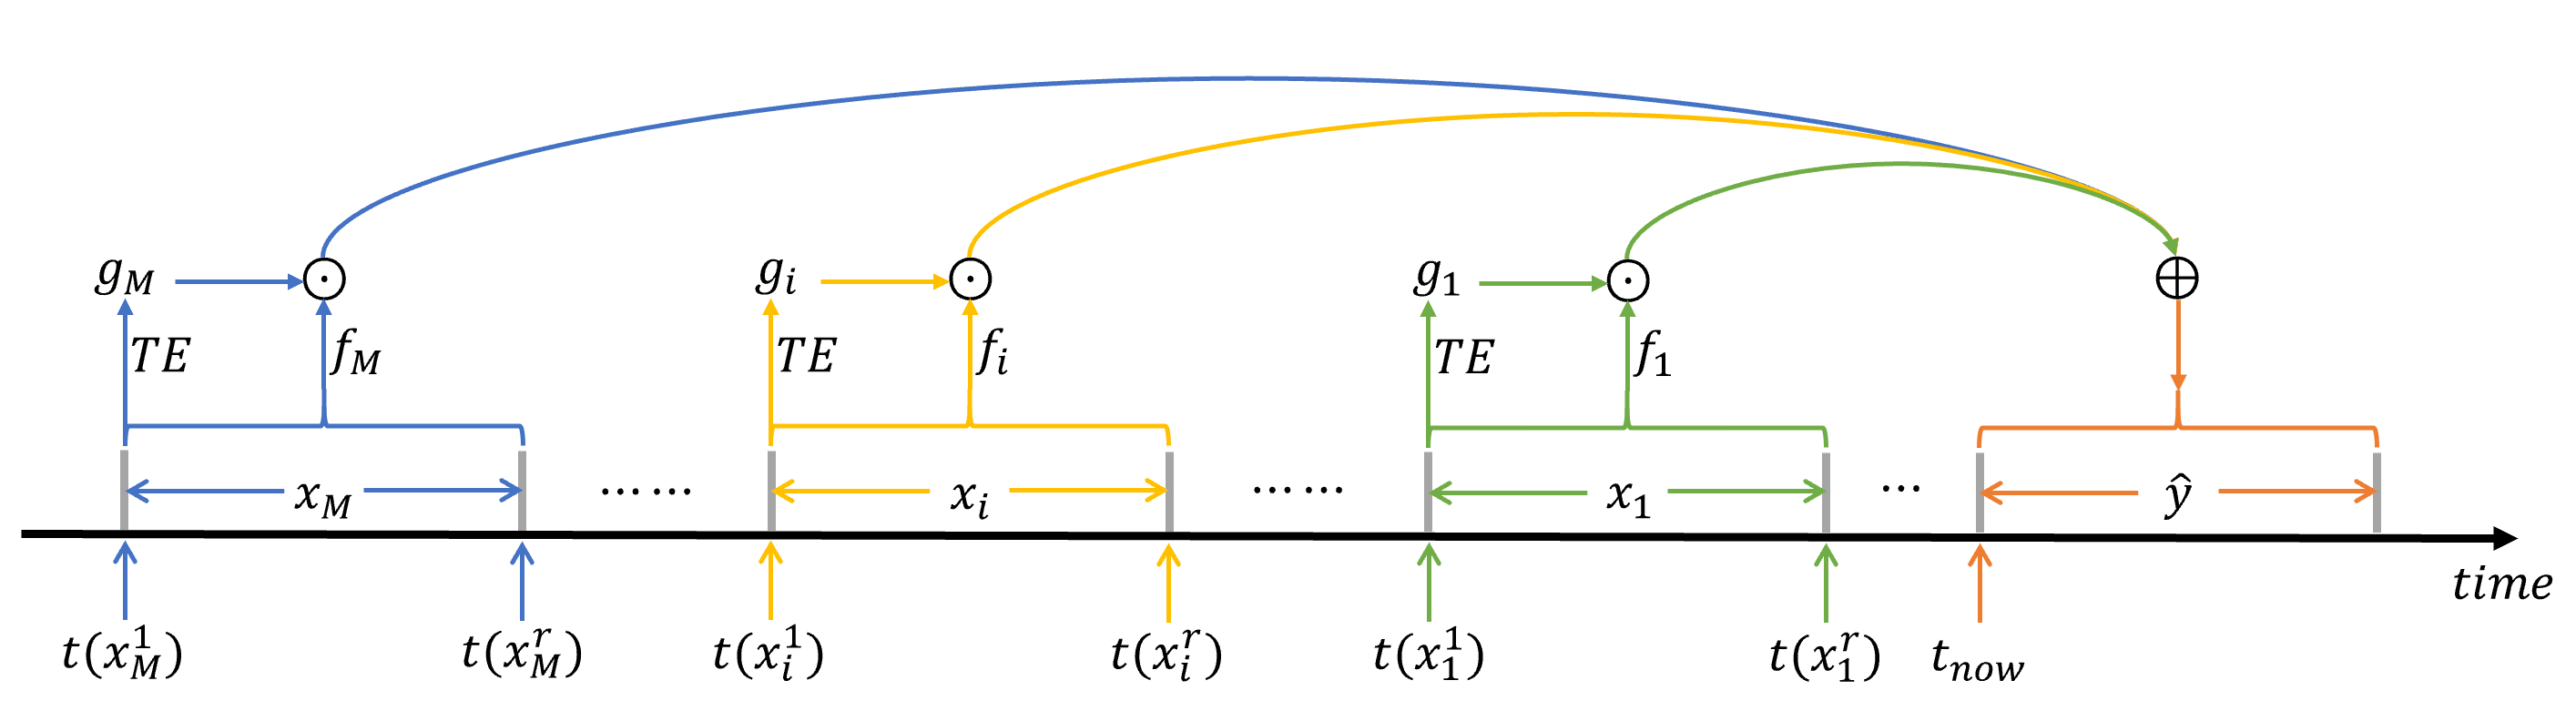
\includegraphics[width=0.48\textwidth]{pictures/Sampling.png}
    \caption{Illustration of the sampling window that slides over the entire time-series graph signals}
    \label{fig:sampling}
\end{figure}

Meanwhile, when the specified present moment $t_{now}$ moving over the whole observed historical graph signals along the time axis, the past $P$ time steps together with the next  $Q$ time steps form a sliding window to generate training samples for our model. As a result, a rich number of distinct training samples can be flexibly yielded from a small historical time-series data in this manner, which evidently improves the capability of the regression model.

\textit{Time embedding for the gated fusion}. 
It is observed that the traffic conditions at the past distinct time slices have different correlation strengths with that of the same future time slice. Accordingly, we propose to incorporate the time information of each input sequence $x_i$ into its corresponding mapping function $f_i(x_i)$ by adding a timing embedding module (called \textit{TE}) in each \textit{TPC} (shown in Fig.~\ref{fig:framework}), and further leverage a gated fusion mechanism to adaptively merge all sub-models \textit{TPCs} to obtain an ultimate prediction model based on the multi-component structure, i.e., MS-GAT. To be specific, by using one-hot coding, we encode the day-of-week and time-of-day of the starting time point $t(x_i^1)$ of each input sequence $x_i$ into the vectors $D_i \in R^7$ and $H_i \in R^{24}$, respectively. After that, by applying a vector embedding approach (e.g., word2vec \cite{church2017word2vec}), the two vectors are transformed to two other vectors with the same dimension, respectively. They are then added together forming the time embedding of the input sequence $x_i$. Formally, the time embedding related to the input sequence $x_i$ corresponds to a tensor denoted as $g_i$, which will be fused as a gate with the associated mapping function $f_i(x_i)$. Thus, the final prediction result after the fusion is:

\begin{equation}
    \label{eqn:gate_fusion}
    \hat{y} = \sum\limits_{i=1}^{M}g_i \odot f_i(x_i),
\end{equation}

where

\begin{equation}
    \label{eqn:time_embedding}
    g_i = TE(D_i, H_i),
\end{equation}

$\odot$ represents the element-wise product, the function $TE(\cdot)$ denotes the specific implementation of the above embedding process related with the timing embedding module called \textit{TE}, both $f_i(\cdot)$ and function $TE(\cdot)$ contain learnable parameters, $g_i \in \mathbb{R}^{C \times N \times Q}$, and $f_i(x_i) \in \mathbb{R}^{C \times N \times Q}$.

\subsection{Multi-dimensional self-attention scheme}
\label{ssec:multi-dimensional_self-attention_scheme}

We first review an ordinary self-attention scheme, called scaled dot-product attention \cite{vaswani2017attention}, which shows excellent performance in learning a specific correlation (e.g., temporal dependency) from sequential data including text, audios and videos. The recent work such as \cite{cai2020traffic, fang2020constgat, park2020st} leveraging the scheme enjoys a great success in dealing with traffic time series data. In this attention scheme, the input and output of a self-attention module that focuses on critical information extraction are fixed to two sequences of vectors, since the scheme adopts ordinary dot-product between vectors as the core operation of whole self-attention process to obtain the correlation strength between input vectors, i.e., \textit{attention score}. To be specific, every element of a sequential data inputted into the self-attention module in turn is a vectorized data, which is typically manipulated into three same vectors called query, key and value respectively, where the key and value are aligned as a key-value pair to represent the information of the current element itself, and the query is applied to calculate the information correlations with all key-value pairs within the sequential data; every element of the resulting sequential data after performing self-attention is also a vectorized data, i.e., each output of the self-attention module, which is computed as a weighted sum of all the values of input sequence, where the weights are the outputs of a \textit{softmax} function, and the inputs of the \textit{softmax} function are scaled dot products of the corresponding queries with all keys. 

\begin{figure}[!ht]
    \centering
    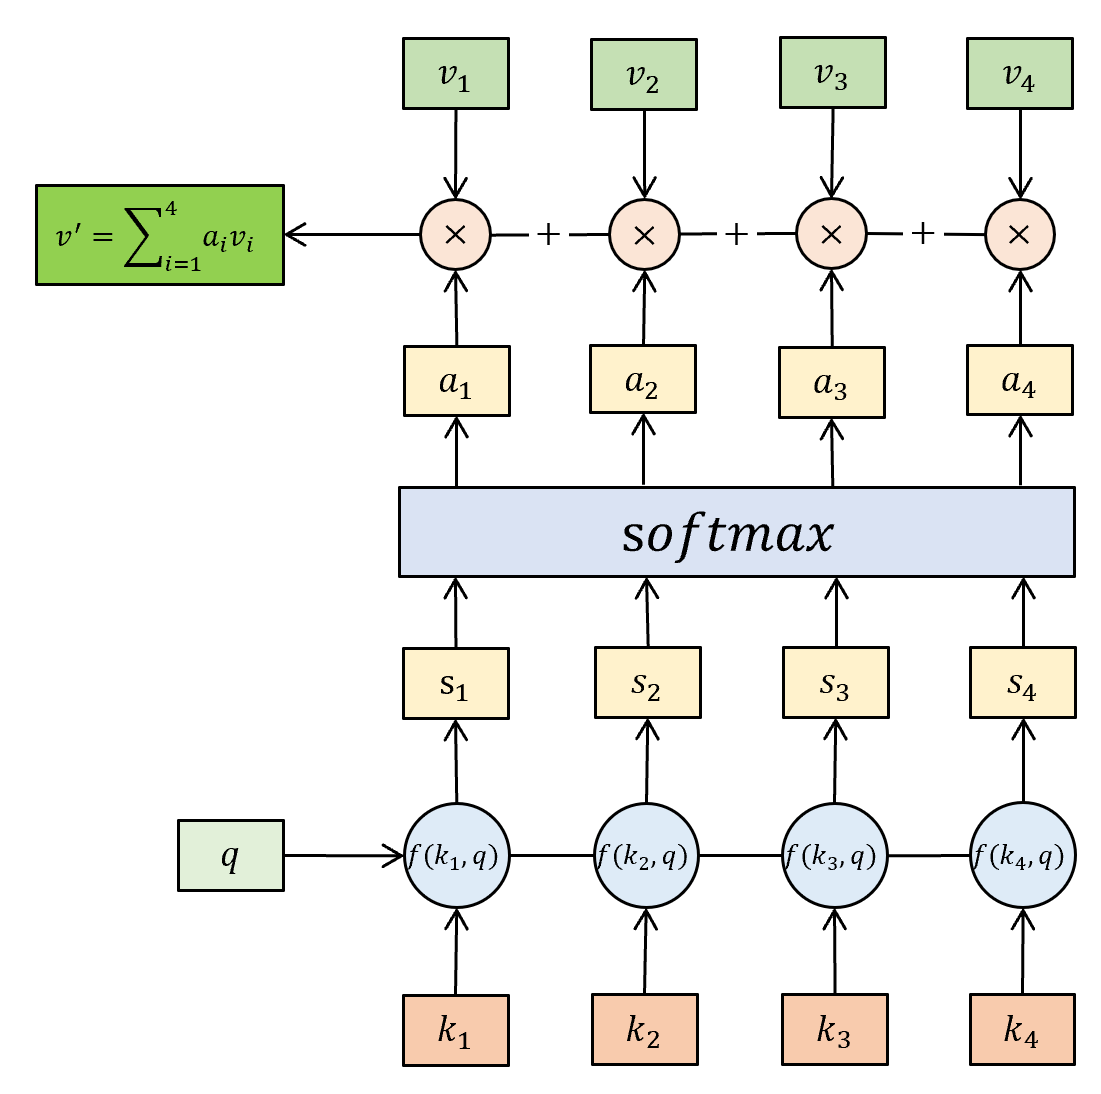
\includegraphics[width=0.32\textwidth]{pictures/Attention.png}
    \caption{The calculation process of self-attention in an exemplar sentence - \textit{this is a cat}. Here, $q$ refers to the \textit{query} vector associated with the word ‘this’, ‘is’, ‘a’ or ‘cat’; $(k_1, v_1)$, $(k_2, v_2)$, $(k_3, v_3)$ and $(k_4, v_4)$ represent the \textit{key-value} pairs of the four separate words respectively; $f$ denotes a type of attention function that adopts dot-product operation between two vectors (i.e., the above \textit{key} and \textit{query}), and $s_1$, $s_2$, $s_3$ and $s_4$ are its resulting attention scores respectively; the $softmax$ function is used to normalize these attention score to $a_1$, $a_2$, $a_3$ and $a_4$ respectively, which are all in the range of $[0, 1]$; $v'$ is the result of current word after performing self-attention by its associated $q$, which contains the contexts of this sentence except for the information of current word itself.}
    \label{fig:attention}
\end{figure}


Taking a linguistic sentence, e.g., \textit{this is a cat}, as an example. Clearly, it is a sequence of words, and can be viewed as a sequential data just over temporal dimension. Importantly, this sentence also conceals the contextual dependencies in temporal dimension between these four separate words. To find out such hidden dependency relations from this sentence, valuable for the tasks of NLP (e.g., language translation), the ordinary attention scheme can be alone applied in a specified information dimension, i.e., temporal dimension of this sequential data. Concretely, each word of the sentence is initially embedded to a vector by a vectorization method (e.g., classic word2vec \cite{church2017word2vec}), and further three same vectors (i.e., query, key and value) derived from the previous vector by linear transform are inputted simultaneously into the self-attention module. After each query of this sentence (i.e., corresponding to each word respectively) accomplishes self-attention operation with all of four key-value pairs, an output sequential data is obtained, which exposes those potential significant contexts into its each sequential element. Figure~\ref{fig:attention} shows the calculation process of this self-attention scheme in the exemplar sentence. Formally, given a query $q$, all keys (packed into matrices $K$) and values (packed into matrices $V$), the output value $value$ is weighted average over the input values as below.

\begin{equation}
    \label{eqn:attention_1}
    value = softmax(\frac{q K^\top}{\sqrt{d_k}}) V
\end{equation}

where $d_k$ is the dimension of $K$. Furthermore, when a sequence of queries is also combined in matrices form $Q$, the attention map, i.e., a resultant matrix including all attention scores, is calculated by Equation~\ref{eqn:attention_2}.

\begin{equation}
    \label{eqn:attention_2}
    Attention(Q,K,V) = softmax(\frac{Q K^\top}{\sqrt{d_k}}) V
\end{equation}

It is clear that the ordinary self-attention scheme receives a vector of the embedding of each element of the input sequence because of the employment of dot-product calculation in the computation of all attention scores. When only two aspects of information in the original input data, e.g., spatial-relevant and temporal-relevant information of normal spatio-temporal data, are attended to, the canonical attention scheme seems easy to carry out in a learning model. In detail, the ordinary scheme typically serializes one aspect of information to be a scalar sequence corresponding to a specific dimension of data (e.g., temporal dimension), while naturally embedding the other aspect of information along the previous dimension one by one into a vector space and further linearly realigning the vector space to another data dimension (e.g., the spatial dimension of spatio-temporal data). The existing traffic prediction models relying on attention mechanism (e.g., \cite{guo2019attention,zheng2020gman}) mostly act in accordance with this scheme. However, if there are more aspects of information to be focused on, the ordinary scheme is not convenient to be deployed. Specifically, when the self-attention is separately paid to each aspect of information, every associated dimension in the input data needs to alternatively apply the above scheme, which would result in such dilemmas as the large parameter scale and the code-level redundancy, thus affecting the model performance. Therefore, we seek a better attention implementation way to capture those correlations when more aspects of information need to be considered from their associated multi-dimensional data.

In MS-GAT, we develop a simple yet effective multi-dimensional self-attention scheme to enable the convenient generalization of existing ordinary self-attention scheme to a multi-dimensional information space and improve the flexibility of handling multi-dimensional data by attention mechanism. Notably, the proposed scheme is formulated as a reusable process, which is very suitable for being universally and conveniently carried out in various information dimension of a multi-dimensional data, even with less computational cost for the resultant model. It works as follows.

\begin{figure}[!ht]
    \centering
    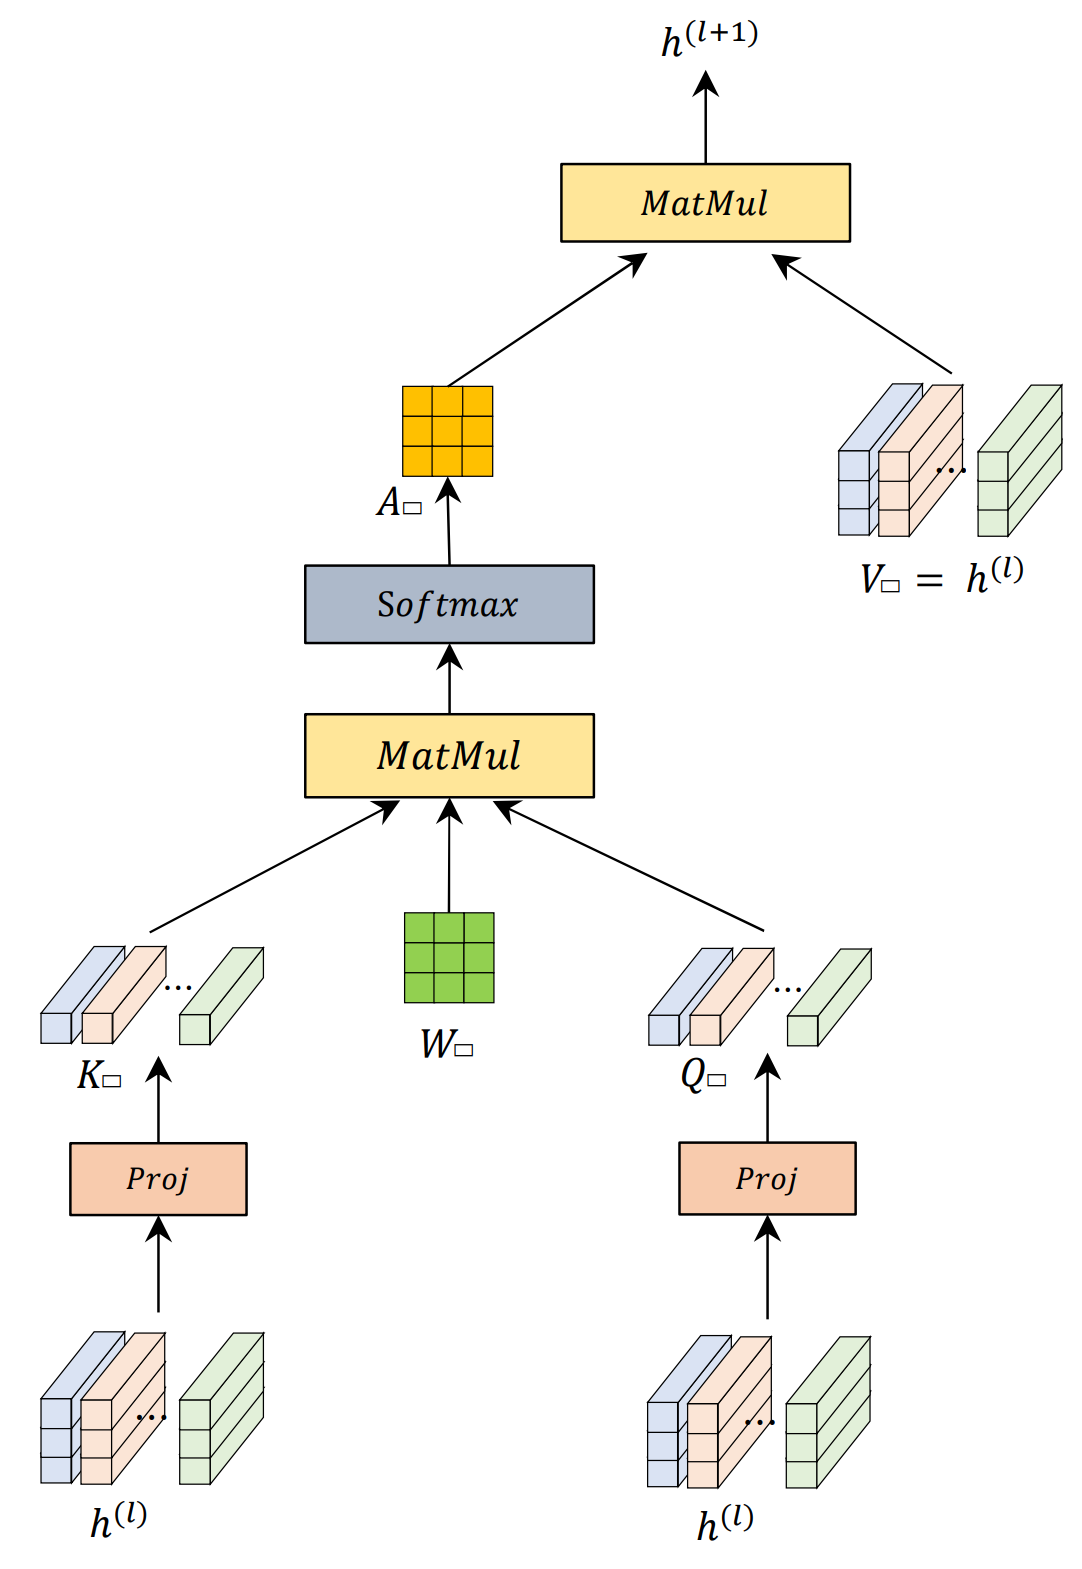
\includegraphics[width=0.4\textwidth]{pictures/Multidim_Attention.png}
    \caption{Illustration of the calculation process of our multi-dimensional self-attention scheme. Here, \textit{MatMul} refers to matrix multiplication; \textit{Proj} denotes the operation of linear transformation; $Q_{_\square}$, $K_{_\square}$ and $V_{_\square}$ are the query, key and value in the multi-dimensional self-attention respectively; $h^{(l)}$ and $h^{(l+1)}$ are the input and output of the $l^{th}$ layer multi-dimensional self-attention. }
    \label{fig:multidim_attention}
\end{figure}

Taking a three-dimensional space including the $x-$, $y-$ and $z-$axes as an example, which represent three different aspects of information associated with the original data, respectively. As a matter of fact, x-axis, y-axis and z-axis can correspond to the spatial, temporal and channel dimensions of spatio-temporal traffic signal data respectively. For the ease of description, the exemplar data space is denoted as a discrete set $\{h_{x,y,z}\}$, each element  $h_{x,y,z}$ is represented in a three-dimensional subscript form. Suppose that the potential correlation inside the information along the $x-$axis needs to be caught, the information separately along the other two dimensions  $y-$ and $z-$axes will work together to achieve it. To be specific, our self-attention scheme sets query, key and value to the identical matrix denoted as $h_{x,:,:}$, where the subscript "$:$" denotes all elements in the corresponding dimension, rather than the vector in the prior ordinary self-attention scheme. For instance, as for diverse spatio-temporal traffic signals throughout a road network, when only different kinds of traffic signals at a certain traffic node are considered, these traffic signal data (e.g., traffic flow, speed and occupancy at a location) within some time range form such a 2-D matrix called query, key or value, owing to their involved information of both temporal and channel dimensions. In addition, if it is a four-dimensional data space, three of them can be set in the tensor form, and so on for the higher-dimensional space. Afterwards, both query and key are transformed to their associated vectors respectively by employing an efficient linear transformation without parameters for tensor operation (e.g., the general API function \textit{torch.einsum()} can be used for the code implementation in its PyTorch version, or \textit{tf.einsum()} for its TensorFlow version). For instance, the 1-D vector $h_{x,\tau,:}$ or $h_{x,:,\tau}$ acts as the vectorization of its associated 2-D matrix $h_{x,:,:}$, where $\tau$ refers to performing the above linear transformation in the second or third dimension. All the vectorized queries and keys are further packed into matrices $Q_{_\square}$ and $K_{_\square}$, respectively (here, the subscript ${_\square}$ is a subscript placeholder for our subsequent formulas in the paper, e.g., Equation~\ref{eqn:graph_attention}). Then, our attention map related to the current dimension, i.e., the correlation strength quantifying the interdependencies between information itself along the $x-$axis is obtained through calculating all related attention scores in parallel by Equation~\ref{eqn:attention_3}.

\begin{equation}
    \label{eqn:attention_3}
    A_{_\square} = Attention(Q_{_\square}, K_{_\square}) = softmax(Q_{_\square} W_{_\square} K_{_\square}^\top)
\end{equation}

where $W_{_\square}$ is an $n_k \times n_k$ matrix that denotes all learnable parameters for applying attention mechanism in the $x-$dimension, and $n_k$ is the number of current keys. Definitely, too large $n_k$ will increase the computational cost of applying the attention, thus impacting on the performance and usage of the resultant model. Thereby, while ensuring sufficient attention-relevant information through providing more keys in our self-attention process, we adopt an effective trick to evade the computational difficulty caused by too much parameters in applying the attention. Specifically, the parameter matrix $W_{_\square}$ is replaced with the multiplication of a small-size learnable parameter matrix and its transposed matrix, i.e., $W_{_\square} = E_{_\square} E_{_\square}^\top$, where $E_{_\square}$ refers to the new matrix with smaller parameter scale $n_k \times e_k$ (here, $e_k < n_k$). Lastly, all values on the current dimension (i.e., the $x-$axis) are renewed to their respective hidden states in parallel by calculating the corresponding weighted sums of all the values based on the current attention map $A_{_\square}$. Figure~\ref{fig:multidim_attention} illustrates the calculation process of our multi-dimensional self-attention scheme. Furthermore, since the above self-attention process on the $x-$axis can be easily developed to a reusable code-level module, it can be also conveniently deployed to the $y-$ or $z-$axis, even to the other new information dimensions in a higher-dimensional data space. Thus, our self-attention scheme can save the development cost by reducing the code-level redundancy.

\subsection{MEAM: multi-relational embedding abreast module}
As the core module of \textit{TPC}, the multi-relational embedding abreast module (MEAM) comprises three abreast embedding branches, which encode the spatial, temporal, and channel relations, respectively. The right part of Fig.~\ref{fig:framework} shows the MEAM architecture. The MEAM stacking replicas are dedicated to extracting the deep features related to the complicated spatial-temporal dynamics of traffic conditions. In each MEAM, the embeddings obtained from separate branches are concatenated into the next-layer MEAM, which attends to implicitly compute their respective importance to the predicted results by the self-attention mechanism of next-layer MEAM. Consequently, the respective contributions of the spatial, temporal and channel relations to the resultant traffic conditions for real-world forecasting can be adaptively distinguished in the whole deep regression model. Moreover, the residual structure \cite{he2016deep} is likewise adopted in MEAM to train the model.

\subsubsection{Spatial relation embedding}
The left branch in MEAM serves for generating the embedding related to spatial relations (i.e., spatial relation extraction shown in Fig.~\ref{fig:core}), which consists of two important operations \textit{GAttention} and \textit{GCN}. The \textit{GAttention} operation first deploys our proposed multi-dimensional self-attention scheme on the spatial dimension of the input data of each MEAM. Take the $j-$layer MEAM in the $i^{th}$ \textit{TPC} of MS-GAT as an example, its input is denoted as $h^{(j-1)} \in \mathbb{R}^{C_j \times N_j \times T_j}$, where $h^{(0)} = x_i$, and $C_j$, $N_j$, and $T_j$ correspond to the channel, spatial and temporal dimensions of $h^{(j-1)}$, respectively. Here, $j$ refers to the identification number of a layer in MEAM stacking replicas. The query, key and value of each spatial node are set to an identical matrix as described in Section IV.B. Then, all the queries and keys are encoded to their associated matrices denoted as $Q_s \in \mathbb{R}^{N_j \times T_j}$ and $K_s \in \mathbb{R}^{N_j \times T_j}$. According to Equation~\ref{eqn:attention_3}, a new matrix $A_s^{(j)} \in \mathbb{R}^{N_j \times N_j}$, reflecting the potential spatial relations, is generated. The \textit{GAttention} operation is defined as follows:

\begin{equation}
    \label{eqn:graph_attention}
    \begin{aligned}
        GAttention(h^{(j-1)}) = A_s^{(j)} & = Attention(Q_s, K_s)      \\
                                          & = softmax(Q_s W_s K_s^\top)
    \end{aligned}
\end{equation}

where $W_s \in \mathbb{R}^{T_j \times T_j}$ refers to a learnable parameter matrix for the attention on the spatial dimension.

Based on the generated $A_s^{(j)}$, we further apply the \textit{GCN} operation to aggregate the hidden states of each node and its first-order neighbors in the MEAM of the previous layer $h^{(j-1)}$. The \textit{GCN} operation is formulated as follows:

\begin{equation}
    \label{eqn:graph_convolution}
    GCN(h^{(j-1)}) =\sigma(\hat{A}_s^{(j)} h^{(j-1)} W_G^{(j)} + b_G^{(j)})
\end{equation}

where $\hat{A}_s^{(j)}=A_s^{(j)} A \in \mathbb{R}^{N_j \times N_j}$ denotes an improved adjacency matrix for subsequent graph convolutional operation, $W_G^{(j)} \in \mathbb{R}^{(C_j \times T_j) \times (C_j \times T_j)}$ and $b_G^{(j)}  \in \mathbb{R}^{(C_j \times T_j)}$ are the learnable parameters for first-order graph convolutional networks \cite{kipf2016semi} in the $j-$layer MEAM, $\sigma$ denotes the activation function, e.g., classic ReLU. After that, the embedding related to spatial relations $e_s^{(j)}=GCN(h^{(j-1)})$ is generated, which is then fused with the results of the other two embedding branches as the input of next-layer MEAM $h^{(j)}$. Note that, during the learning process of the current MEAM, the importance of the previous layer's spatial embedding $e_s^{(j-1)}$ to the prediction results has been synchronously learned in an implicit manner by performing self-attention on the channel and temporal dimensions of $h^{(j-1)}$.

\subsubsection{Temporal relation embedding}
In a real-world road network, there are typically explicit or implicit temporal relations between pair-wise traffic conditions at different timestamps. For example, the traffic speeds on an identical traffic node might present daily-periodic or weekly-periodic trends. Also, the current average vehicle speed on a node could be associated with the traffic volume at a past timestamp on another node. To this end, we build an independent branch in MEAM to focus on the embedding of such temporal relations (i.e., temporal relation extraction shown in Fig.~\ref{fig:core}).

The embedding branch also comprises two critical operations \textit{TAttention} and \textit{TCN}. The \textit{TAttention} operation is similar to the aforementioned \textit{GAttention} operation. Their difference is that  \textit{TAttention}  realizes our proposed multi-dimensional self-attention scheme on the temporal dimension of the input data of each MEAM. Let us further take the $j-$layer MEAM in the $i^{th}$ \textit{TPC} of MS-GAT as an example, according to Equation~\ref{eqn:attention_3}, a temporal attention map $A_T^{(j)} \in \mathbb{R}^{T_j \times T_j}$ is obtained to semantically represent the pair-wise correlation strengths between the traffic conditions at different timestamps. The \textit{TAttention} operation is defined as follows:

\begin{equation}
    \label{eqn:temporal_attention}
    \begin{aligned}
        TAttention(h^{(j-1)})  = A_T^{(j)} & = Attention(Q_T, K_T)      \\
                                           & = softmax(Q_T W_T K_T^\top)
    \end{aligned}
\end{equation}

where $Q_T \in \mathbb{R}^{T_j \times N_j}$ and $K_T \in \mathbb{R}^{T_j \times N_j}$ refer to the query and key matrices of temporal attention respectively, $W_T \in \mathbb{R}^{N_j \times N_j}$ is its learnable weight matrix. Considering that the number of traffic nodes straightly affects the parameter scale of the weight matrix of temporal attention, we adopt the trick mentioned in Section~\ref{ssec:multi-dimensional_self-attention_scheme} to balance the efficiency and accuracy of our attention-based model. Thus, the \textit{TAttention} operation is further formulated as follows:

\begin{equation}
    \label{eqn:trick_temporal_attention}
    \begin{aligned}
        TAttention(h^{(j-1)}) & = A_T^{(j)}                        \\
                              & = Attention(Q_T, K_T)              \\
                              & = softmax(Q_T E_T E_T^\top K_T^\top)
    \end{aligned}
\end{equation}

where $E_T \in \mathbb{R}^{N_j \times d_E}$ and $d_E$ denotes a number much smaller than $N_j$.

Subsequently, the input of this embedding branch (equivalent to the input of the current MEAM $h^{(j-1)}$) is taken as the value of the temporal attention, which is then renewed to $h_T^{(j-1)} \in \mathbb{R}^{C_j \times N_j \times T_j}$ by leveraging the obtained temporal attention map $A_T^{(j)}$. We further perform the \textit{TCN} operation to deal with $h_T^{(j-1)}$ along its temporal dimension. \textit{TCN} follows the idea of temporal convolutional networks \cite{bai2018empirical} to  preserve the chronological order of data (namely the outputs at the current time are only related to its historical data). To be specific, two levels of dilated causal convolutions are applied to represent $h_T^{(j-1)}$. A single dilated causal convolution operation $F$ on element $\xi$ of the time-series data $h_T^{(j-1)}(v)$ at a traffic node $v$ takes the following form:

\begin{equation}
    \label{eqn:dilated_causal_convolution}
    \begin{aligned}
        F(\xi) = \sum_{m=0}^{\pi-1} \phi_m \cdot [h_T^{(j-1)}(v)]_{\xi-\omega \cdot m}
    \end{aligned}
\end{equation}

where $\omega$ is the dilation factor, $\phi_m$ is our \textit{TCN} filter, $\pi$ is its size, and $\xi-\omega \cdot m$ accounts for the direction of the past. In practice, we utilize the zero padding strategy to keep the temporal length unchanged. At the end, the temporal embedding $e_T^{(j)}$ is obtained.

\subsubsection{Channel relation embedding}
Besides the two previous embedding branches, we build another separate branch in MEAM for the embedding of our proposed channel relations in traffic networks (i.e., channel relation extraction shown in Fig.~\ref{fig:core}). This embedding branch is primarily implemented by the \textit{CAttention} operation to pick up the pairwise correlations between channels by a self-attention mechanism. Specifically, \textit{CAttention}  carries out our proposed multi-dimensional self-attention scheme on the channel dimension of the input data of each MEAM, while the information situated in the other two dimensions will jointly attend to the computation of the attention score between different traffic conditions along the channel dimension. To a certain extent, the attention score semantically represents the correlation strength between channels. Accordingly, also for the $j-$layer MEAM in the $i^{th}$ \textit{TPC} of MS-GAT, the channel attention map associated with the input of this branch, denoted as $A_c^{(j)} \in \mathbb{R}^{C_j \times C_j}$, is computed by:

\begin{equation}
    \label{eqn:channel_attention}
    \begin{aligned}
        CAttention(h^{(j-1)})  = A_c^{(j)} & = Attention(Q_c, K_c)      \\
                                           & = softmax(Q_c W_c K_c^\top)
    \end{aligned}
\end{equation}

where $Q_c \in \mathbb{R}^{C_j \times T_j}$ and $K_c \in \mathbb{R}^{C_j \times T_j}$ are the query and key matrices of the channel attention respectively, $W_c \in \mathbb{R}^{T_j \times T_j}$ indicates its learnable weight matrix. Afterward, we set the input of this embedding branch (equal to the input of the current MEAM $h^{(j-1)}$ as the value of our channel attention, which can thus be renewed by applying the obtained channel attention map $A_c^{(j)}$. Finally, the channel embedding $e_c^{(j)}$ is generated after the necessary dimension transformation by the $1 \times 1$ convolution. Likewise, its importance weight to the prediction results will be implicitly evaluated in the MEAM of the next layer.
\section{Experiments}
\label{sec:experiments}
In this section, extensive experiments are conducted to verify the effectiveness and superiority of the proposed MS-GAT\footnote{The code is available at: \url{https://github.com/luokn/ms-gat}.}.

\subsection{Experiment setup}
\subsubsection{Data description}
We evaluate the performance of MS-GAT on five public traffic network datasets: the PEMS-BAY dataset  \cite{li2017diffusion} and the PEMSD3, PEMSD4, PEMSD7 and PEMSD8 datasets  \cite{song2020spatial}. They were all constructed from the Caltrans Performance Measurement System (PeMS) \cite{chen2001freeway} and are commonly used in traffic prediction. Each of these five datasets is associated with a district of California, i.e., corresponding to a separate traffic road network, respectively. All time-series readings in these datasets are aggregated into 5-minute windows, which means there are 12 sampling points (i.e., timesteps) for every hour. Table I shows the related information of the five datasets. Note that, PEMSD4, PEMSD8 and PEMS-BAY contain three kinds of traffic signals (indicators) at each node: traffic flow, average speed and average occupancy, whereas PEMSD3 and PEMSD7 just involve the traffic flow.

\begin{table}[!htb]
    \caption{The Data description and statistics.}
    \label{tab:datasets}
    \centering
    \begin{tabular}{ccccc}
        \toprule[2pt]
        Datasets & \#Nodes & \#Edges & \#TimeSteps & \#Channels \\
        \hline
        PEMSD3   & 358     & 547     & 26208       & 1          \\
        PEMSD4   & 307     & 340     & 16992       & 3          \\
        PEMSD7   & 883     & 866     & 28224       & 1          \\
        PEMSD8   & 170     & 295     & 17856       & 3          \\
        PEMS-BAY & 325     & 8033    & 52116       & 3          \\
        \bottomrule[2pt]
    \end{tabular}
\end{table}

For each dataset, we derive a spatial adjacency matrix based on the connectivity among traffic nodes, and adopt z-score normalization to standardize all the data. Meanwhile, our data augmentation method (see details in Section~\ref{ssec:the_network_architecture}) is applied to the five datasets separately. After that, we split the data from the five datasets respectively with the same ratio 6:2:2 into training, validation and test sets.

\subsubsection{Baseline methods}
Six state-of-the-art models are compared with MS-GAT for performance evaluation. As shown in \cite{song2020spatial,mengzhang2020spatial}, the baseline methods based on deep neural networks (DNN) exhibit more superior traffic prediction results than traditional time-series methods such as HA \cite{liu2004summary}, ARIMA \cite{williams2003modeling}, VAR \cite{zivot2006vector} and SVR \cite{1364002}. In particular, they achieve the impressive prediction results by exploiting the generalized DNN on graphs. Thus, our experiments select the following six representative graph networks as the baselines: DCRNN, STGCN, ASTGCN, Graph WaveNet, STSGCN and AGCRN, where STSGCN and AGCRN are the recent approaches.  

DCRNN: A Diffusion Convolutional Recurrent Neural Network \cite{li2017diffusion}, which leverages the diffusion graph convolutional networks and the encoder-decoder recurrent neural networks to capture spatial dependencies and temporal dependencies in the traffic flow, respectively.

STGCN: A Spatio-Temporal Graph Convolutional Network \cite{yu2017spatio}, which combines graph convolution with 1-D convolution to model the spatial and temporal dynamics of the traffic flow.

ASTGCN: An Attention-based Spatial Temporal Graph Convolutional Network \cite{guo2019attention}, which introduces attention mechanisms into the spatial-temporal modeling of traffic flow based on graph convolutional networks and also adopts multi-component structure.

Graph WaveNet: It refers to the method in \cite{wu2019graph}, which develops an adaptive dependency matrix and combines it into graph convolution with dilated casual convolution to capture spatial-temporal dependencies.

STSGCN: A Spatial-Temporal Synchronous Graph Convolutional Network \cite{song2020spatial}, which exploits a spatial-temporal graph convolutional module to synchronously capture the localized spatial-temporal correlations directly.

AGCRN: An Adaptive Graph Convolutional Recurrent Network \cite{bai2020adaptive}, which captures fine-grained spatial and temporal correlations in traffic series automatically based on recurrent networks and two adaptive modules that enhance GCN with new capabilities. 

\subsubsection{Evaluation metrics}
To make fair comparison, we deploy three commonly-used metrics to measure the difference between the ground truth and the predicted traffic flow, which are mean absolute error (MAE), root mean square error (RMSE), and mean absolute percentage error (MAPE), respectively. Suppose that $\mathcal{Y}_{m,n}$ represents the ground truth, $\hat{\mathcal{Y}}_{m,n}$ represents the predicted value (here, $1 \leq m \leq N$, $1 \leq n \leq Q$, $N$ denotes the number of traffic nodes, and $Q$ denotes the future time steps), and the three metrics are defined as follows:

\begin{equation}
    \label{eqn:mae}
    MAE = \frac{1}{NQ} \sum\limits_{m=1}^{N}\sum\limits_{n=1}^{Q} \left | \mathcal{Y}_{m,n} - \hat{\mathcal{Y}}_{m,n} \right |
\end{equation}

\begin{equation}
    \label{eqn:rmse}
    RMSE = \sqrt{\frac{1}{NQ} \sum\limits_{m=1}^{N}\sum\limits_{n=1}^{Q} \left ( \mathcal{Y}_{m,n} - \hat{\mathcal{Y}}_{m,n} \right )^2}
\end{equation}

\begin{equation}
    \label{eqn:mape}
    MAPE = \frac{1}{NQ} \sum\limits_{m=1}^{N}\sum\limits_{n=1}^{Q} \left | \frac{ \mathcal{Y}_{m,n} - \hat{\mathcal{Y}}_{m,n}}{\mathcal{Y}_{m,n}} \right | \times 100 \%
\end{equation}

\subsubsection{The MS-GAT settings}
We implement the MS-GAT model using PyTorch \cite{ketkar2017introduction}. MS-GAT takes multi-segment historical data as input according to the number of its prediction components (i.e., \textit{TPCs}). Each segment of the whole input samples of MS-GAT has fixed timesteps that is set to 12. Accordingly, every group of the spatial-temporal data of the past hour is assigned to a separate prediction component of MS-GAT, which could be any hour in the historically observed data, e.g., an hour, the second hour or the third hour before the forecasting time point, or one hour of the day before the forecasting time point, one hour of the week before the forecasting time point. In the experiments, we use MS-GAT to predict the traffic flow of one hour, half an hour and a quarter of an hour in the future. Meanwhile, we choose Huber loss \cite{huber1992robust} as the lose function, which is less sensitive to outliers than the squared error loss, which is defined below:

\begin{equation}
    \label{eqn:huber_loss}
    \mathcal{L}_{\delta}(\mathcal{Y}, \hat{\mathcal{Y}}) =
    \begin{aligned}
        \begin{cases}
            \frac{1}{2} \left ( \mathcal{Y} - \hat{\mathcal{Y}} \right ) ^2                 & if \ \left | \mathcal{Y} - \hat{\mathcal{Y}} \right | \leq \delta \\
            \delta \left | \mathcal{Y} - \hat{\mathcal{Y}} \right | - \frac{1}{2} \delta ^2 & otherwise
        \end{cases}
    \end{aligned}
\end{equation}

where $\mathcal{Y}$ denotes the ground truth, $\hat{\mathcal{Y}}$ denotes the predicted value, and $\delta$ is the hyperparameter to control the sensitivity of squared error loss that is set to 40 in our experiments.
We train MS-GAT using the Adam optimizer with learning rate 0.001, and the training epoch is set to 100. MS-GAT is evaluated more than 8 times on each dataset. Moreover, all experiments are conducted on a 64-bit Ubuntu 18.04 computer with two CPUs (Intel Xeon Platinum 8176 @2.10 GHz, 312 GB memory) and eight GPUs (NVIDIA GeForce RTX 2080 TI, 11 GB memory).

\subsection{Comparison results and analysis}

\begin{table*}[!htb]
    \caption{Performance comparison of MS-GAT and baseline models on PEMSD3, PEMSD4, PEMSD7 and PEMSD8.}
    \label{tab:pemsd3-8}
    \centering
    \scalebox{0.9}{
        \begin{tabular}{cccccccccc}
            \toprule[2pt]
            \multirow{2}{*}{Datasets}                    &
            \multirow{2}{*}{Metric}                      &
            \multirow{2}{*}{DCRNN}                       &
            \multirow{2}{*}{STGCN}                       &
            \multirow{2}{*}{ASTGCN(r)}                   &
            \multirow{2}{*}{Graph WaveNet}               &
            \multirow{2}{*}{STSGCN}                      &
            \multirow{2}{*}{AGCRN}                       &
            \multirow{2}{*}{\textbf{MS-GAT}}                                                                                                                                                                                                          
            \\
            \\
            \hline
            \multicolumn{1}{c|}{\multirow{3}{*}{PEMSD3}} & \multicolumn{1}{c|}{MAE}      & 18.18 $\pm$ 0.15 & 17.49 $\pm$ 0.46 & 17.69 $\pm$ 1.43 & 19.85 $\pm$ 0.03 & 17.48 $\pm$ 0.15 & 16.13 $\pm$ 0.19 & \textbf{15.68 $\pm$ 0.24} \\
            \multicolumn{1}{c|}{}                        & \multicolumn{1}{c|}{MAPE(\%)} & 18.91 $\pm$ 0.82 & 17.15 $\pm$ 0.45 & 19.40 $\pm$ 2.24 & 19.31 $\pm$ 0.49 & 16.78 $\pm$ 0.20 & -                & \textbf{16.11 $\pm$ 0.13} \\
            \multicolumn{1}{c|}{}                        & \multicolumn{1}{c|}{RMSE}     & 30.31 $\pm$ 0.25 & 30.12 $\pm$ 0.70 & 29.66 $\pm$ 1.68 & 32.94 $\pm$ 0.18 & 29.21 $\pm$ 0.56 & 28.42 $\pm$ 0.07 & \textbf{26.54 $\pm$ 0.16} \\
            \hline
            \multicolumn{1}{c|}{\multirow{3}{*}{PEMSD4}} & \multicolumn{1}{c|}{MAE}      & 24.70 $\pm$ 0.22 & 22.70 $\pm$ 0.64 & 22.93 $\pm$ 1.29 & 25.45 $\pm$ 0.03 & 21.19 $\pm$ 0.10 & 19.75 $\pm$ 0.11 & \textbf{19.54 $\pm$ 0.19} \\
            \multicolumn{1}{c|}{}                        & \multicolumn{1}{c|}{MAPE(\%)} & 17.12 $\pm$ 0.37 & 14.59 $\pm$ 0.21 & 16.56 $\pm$ 1.36 & 17.29 $\pm$ 0.24 & 13.90 $\pm$ 0.05 & 13.00 $\pm$ 0.18 & 13.44 $\pm$ 0.28          \\
            \multicolumn{1}{c|}{}                        & \multicolumn{1}{c|}{RMSE}     & 38.12 $\pm$ 0.26 & 35.55 $\pm$ 0.75 & 35.22 $\pm$ 1.90 & 39.70 $\pm$ 0.04 & 33.65 $\pm$ 0.20 & 32.41 $\pm$ 0.20 & \textbf{31.69 $\pm$ 0.15} \\
            \hline
            \multicolumn{1}{c|}{\multirow{3}{*}{PEMSD7}} & \multicolumn{1}{c|}{MAE}      & 25.30 $\pm$ 0.52 & 25.38 $\pm$ 0.49 & 28.05 $\pm$ 2.34 & 26.85 $\pm$ 0.05 & 24.26 $\pm$ 0.14 & 21.19 $\pm$ 0.09 & \textbf{20.47 $\pm$ 0.13} \\
            \multicolumn{1}{c|}{}                        & \multicolumn{1}{c|}{MAPE(\%)} & 11.66 $\pm$ 0.33 & 11.08 $\pm$ 0.18 & 13.92 $\pm$ 1.65 & 12.12 $\pm$ 0.41 & 10.21 $\pm$ 1.65 & 8.95 $\pm$ 0.08  & \textbf{8.84 $\pm$ 0.14}  \\
            \multicolumn{1}{c|}{}                        & \multicolumn{1}{c|}{RMSE}     & 38.58 $\pm$ 0.70 & 38.78 $\pm$ 0.58 & 42.57 $\pm$ 3.31 & 42.78 $\pm$ 0.07 & 39.03 $\pm$ 0.27 & 35.12 $\pm$ 0.12 & \textbf{34.17 $\pm$ 0.08} \\
            \hline
            \multicolumn{1}{c|}{\multirow{3}{*}{PEMSD8}} & \multicolumn{1}{c|}{MAE}      & 17.86 $\pm$ 0.03 & 18.02 $\pm$ 0.14 & 18.61 $\pm$ 0.40 & 19.13 $\pm$ 0.08 & 17.13 $\pm$ 0.09 & 16.10 $\pm$ 0.11 & \textbf{14.78 $\pm$ 0.09} \\
            \multicolumn{1}{c|}{}                        & \multicolumn{1}{c|}{MAPE(\%)} & 11.45 $\pm$ 0.03 & 11.40 $\pm$ 0.10 & 13.08 $\pm$ 1.00 & 12.68 $\pm$ 0.57 & 10.96 $\pm$ 0.07 & 10.27 $\pm$ 0.08 & \textbf{10.07 $\pm$ 0.12} \\
            \multicolumn{1}{c|}{}                        & \multicolumn{1}{c|}{RMSE}     & 27.83 $\pm$ 0.05 & 27.83 $\pm$ 0.20 & 28.16 $\pm$ 0.48 & 31.05 $\pm$ 0.07 & 26.80 $\pm$ 0.18 & 25.62 $\pm$ 0.17 & \textbf{24.15 $\pm$ 0.07} \\
           \bottomrule[2pt]
        \end{tabular}
    }
\end{table*}

\begin{table*}[!htb]
    \caption{Performance comparison of MS-GAT and baseline models on PEMS-BAY.}
    \label{tab:pems-bay}
    \centering
    \begin{tabular}{ccccccccc}
        \toprule[2pt]
        \multirow{2}{*}{Dataset}                    &
        \multirow{2}{*}{Metric}                     &
        \multirow{2}{*}{DCRNN}                      &
        \multirow{2}{*}{STGCN}                      &
        \multirow{2}{*}{Graph WaveNet}              &
        \multirow{2}{*}{STSGCN}                     &
        \multirow{2}{*}{STGCNN}                     &
        \multirow{2}{*}{AGCRN}                      &
        \multirow{2}{*}{\textbf{MS-GAT}}                                                                                                        
        \\
        \\
        \hline
        \multicolumn{1}{c|}{\multirow{3}{*}{15min}} & \multicolumn{1}{c|}{MAE}      & 1.38 & 1.36 & 1.30 & 2.54 & 1.20 & 1.16 & \textbf{1.13 $\pm$ 0.02} \\
        \multicolumn{1}{c|}{}                       & \multicolumn{1}{c|}{MAPE(\%)} & 2.90 & 2.90 & 2.73 & 5.88 & 2.34 & 2.47 & \textbf{2.44 $\pm$ 0.06} \\
        \multicolumn{1}{c|}{}                       & \multicolumn{1}{c|}{RMSE}     & 2.95 & 2.96 & 2.74 & 4.79 & 2.43 & 2.40 & \textbf{2.38 $\pm$ 0.04} \\
        \hline
        \multicolumn{1}{c|}{\multirow{3}{*}{30min}} & \multicolumn{1}{c|}{MAE}      & 1.74 & 1.81 & 1.63 & 2.60 & 1.46 & 1.41 & \textbf{1.35 $\pm$ 0.01} \\
        \multicolumn{1}{c|}{}                       & \multicolumn{1}{c|}{MAPE(\%)} & 3.90 & 4.17 & 3.67 & 6.03 & 3.09 & 3.12 & \textbf{3.09 $\pm$ 0.04} \\
        \multicolumn{1}{c|}{}                       & \multicolumn{1}{c|}{RMSE}     & 3.97 & 4.27 & 3.70 & 4.93 & 3.27 & 3.10 & \textbf{2.94 $\pm$ 0.02} \\
        \hline
        \multicolumn{1}{c|}{\multirow{3}{*}{60min}} & \multicolumn{1}{c|}{MAE}      & 2.07 & 2.49 & 1.95 & 2.71 & 1.83 & 1.79 & \textbf{1.74 $\pm$ 0.03} \\
        \multicolumn{1}{c|}{}                       & \multicolumn{1}{c|}{MAPE(\%)} & 4.90 & 5.79 & 4.63 & 6.39 & 4.15 & 4.01 & \textbf{3.97 $\pm$ 0.05} \\
        \multicolumn{1}{c|}{}                       & \multicolumn{1}{c|}{RMSE}     & 4.74 & 5.69 & 4.52 & 5.28 & 3.20 & 3.78 & 3.88 $\pm$ 0.02          \\
        \bottomrule[2pt]
    \end{tabular}
\end{table*}

Table~\ref{tab:pemsd3-8} and Table~\ref{tab:pems-bay} present the performance comparison between different models on the commonly-used datasets. Table~\ref{tab:pemsd3-8} shows MS-GAT outperforms baselines consistently on the PEMSD3, PEMSD4, PEMSD7 and PEMSD8 datasets. For instance, MS-GAT achieves 7.0\%, 1.4\%, 7.8\% and 12.6\% improvement respectively over the state-of-the-art models on the metric of MAE. Meanwhile, Table~\ref{tab:pems-bay} shows comparison with baselines, MS-GAT consistently achieves the  best results for forecasting 15 minutes, 30 minutes and 1 hour ahead on the PEMS-BAY dataset. It suggests MS-GAT has an effective prediction capability in both short-range and long-range cases. By further comparison, we have the following observations.

On one hand, although the state-of-the-art models gain impressive results by developing different variants of GNN and RNN to deal with the spatial-temporal graph modeling issues for traffic prediction,  their processes of  capturing the spatial and temporal relations are carried out in an alternate manner. Instead, MS-GAT is aware of the couplings between spatial relations and temporal relations and their influence on future traffic conditions, which thus adopts a synchronously handling manner to capture diverse relations hidden in traffic time-series readings. Relying on this synchronous manner for modeling relations, MS-GAT can dynamically assign the importance weight of the spatial, temporal  and channel relations by adaptively learning from the ground-truth. As a result, the leaning ability of the regression model is strengthened, and the comparative results shown in Table~\ref{tab:pemsd3-8} and Table~\ref{tab:pems-bay} also demonstrate that the innovation in MS-GAT is beneficial to improving the accuracy of traffic prediction.

On the other, the model architecture   is critical to the performance of traffic prediction. The comparative experiments show that the predictive models with the multi-component architecture perform significantly better  those without considering multi-components. The reason might be that the multi-component architecture takes advantage of ensemble learning, like what is observed in ASTGCN \cite{guo2019attention} and MS-GAT. However, they work differently. For ASTGCN, first, it adopts ChebNet \cite{defferrard2016convolutional} as a graph convolution operation to model spatial correlations, which makes it inferior to other predictive models using more excellent graph convolution networks, e.g., STSGCN \cite{song2020spatial} and STFGNN \cite{mengzhang2020spatial}. Second, it stacks a standard convolution layer in the temporal dimension to merge the information at the neighboring time slice, which makes it hard to gain a promising ability of modeling temporal correlation as Graph WaveNet \cite{wu2019graph} using dilated casual convolution. Third, it develops a very complicated spatial-temporal attention mechanism to capture the dynamic spatial and temporal correlations in the traffic network, which instead brings about a large amount of model parameters and makes it hard to train and easy to overfit. In contrast, MS-GAT pursues to fill these gaps. Except for designing a distinctive time-gating multi-component architecture, MS-GAT also focuses on the following aspects. First, by utilizing a first-order Chebyshev polynomial to simplify ChebNet \cite{defferrard2016convolutional} as our efficient GCN operation, MS-GAT  significantly reduces the complexity of aggregating spatial information and achieves the approximate effect of ordinary higher-order ChebNet by stacking multiple \textit{GCN} operations in MEAM. Second, MS-GAT employs TCN (i.e., temporal convolutional networks \cite{bai2018empirical}) to capture complex relations between traffic conditions in the temporal dimension rather than using prior CNN- or RNN-based methods (e.g., STGCN \cite{yu2017spatio}). Since TCN has the advantage of causal convolution and more flexible receptive field in sequence modeling, it thus performs better than CNNs and RNNs in aggregating temporal information. Third, MS-GAT emphasizes the significance the channel relations hidden among traffic conditions, which is verified  benefitable for accurate traffic prediction. Lastly, MS-GAT develops a simple yet effective multi-dimensional self-attention scheme to generalize existing ordinary self-attention mechanism to all information dimensions of traffic conditions and to improve the flexibility of handling multi-dimensional data based on attention mechanism. The above analysis explains why MS-GAT performs best in the comparative experiments. Moreover, MS-GAT also maintains a competitive parameter scale that ensures the efficiency of training and performing the prediction.

\subsection{The ablation study}
\begin{table*}[!htb]
    \caption{The ablation study of MS-GAT on PEMSD3, PEMSD4, PEMSD7 and PEMSD8 (best number per row is shown in bold).}
    \label{tab:ablation}
    \centering
    \begin{tabular}{cccccccc}
        \toprule[2pt]
        \multirow{4}{*}{Dataset}                     &
        \multirow{4}{*}{Metrics}                     &
        \multirow{4}{*}{TPC}                         &
        \multirow{2}{*}{TPC $\times$ 2}              &
        \multirow{2}{*}{TPC $\times$ 3}              &
        \multirow{2}{*}{TPC $\times$ 4}              &
        \multirow{2}{*}{TPC $\times$ 5}              &
        \multirow{4}{*}{no CAttention}               
        \\
        \\
        \cline{4-7}
        & & &
        \multirow{2}{*}{without/with TE}             &
        \multirow{2}{*}{without/with TE}             &
        \multirow{2}{*}{without/with TE}             &
        \multirow{2}{*}{without/with TE}             &
        \\
        \\
        \hline
        \multicolumn{1}{c|}{\multirow{3}{*}{PEMSD3}} & \multicolumn{1}{c|}{MAE}      & 18.87 & 16.70/16.25 & 16.38/16.04 & 16.08/\textbf{15.68} & 17.38/16.88          & 15.82 \\
        \multicolumn{1}{c|}{}                        & \multicolumn{1}{c|}{MAPE(\%)} & 32.04 & 17.79/17.55 & 17.22/16.98 & 16.88/\textbf{16.11} & 17.06/17.21          & 16.37 \\
        \multicolumn{1}{c|}{}                        & \multicolumn{1}{c|}{RMSE}     & 29.06 & 27.11/26.74 & 26.87/26.62 & 26.84/\textbf{26.54} & 29.97/29.07          & 27.05 \\
        \hline
        \multicolumn{1}{c|}{\multirow{3}{*}{PEMSD4}} & \multicolumn{1}{c|}{MAE}      & 25.42 & 22.77/20.48 & 21.43/20.30 & 21.42/20.11          & 20.58/\textbf{19.56} & 20.41 \\
        \multicolumn{1}{c|}{}                        & \multicolumn{1}{c|}{MAPE(\%)} & 21.94 & 15.95/14.12 & 15.45/13.70 & 15.24/13.70          & 14.20/\textbf{13.44} & 14.39 \\
        \multicolumn{1}{c|}{}                        & \multicolumn{1}{c|}{RMSE}     & 37.95 & 35.63/32.34 & 33.67/32.17 & 33.61/31.98          & 32.95/\textbf{31.69} & 32.73 \\
        \hline
        \multicolumn{1}{c|}{\multirow{3}{*}{PEMSD7}} & \multicolumn{1}{c|}{MAE}      & 27.86 & 24.40/22.50 & 23.33/22.37 & 23.04/21.55          & 20.84/\textbf{20.47} & 20.76 \\
        \multicolumn{1}{c|}{}                        & \multicolumn{1}{c|}{MAPE(\%)} & 16.18 & 10.66/9.67  & 10.51/9.71  & 10.02/9.35           & 9.13/\textbf{8.84}   & 9.01 \\
        \multicolumn{1}{c|}{}                        & \multicolumn{1}{c|}{RMSE}     & 41.53 & 38.07/35.67 & 36.29/35.64 & 35.95/34.68          & 34.17/\textbf{34.17} & 34.08 \\
        \hline
        \multicolumn{1}{c|}{\multirow{3}{*}{PEMSD8}} & \multicolumn{1}{c|}{MAE}      & 20.63 & 17.68/16.50 & 16.82/16.43 & 16.77/15.71          & 15.34/\textbf{14.78} & 15.65 \\
        \multicolumn{1}{c|}{}                        & \multicolumn{1}{c|}{MAPE(\%)} & 18.89 & 11.44/10.73 & 11.02/10.81 & 11.32/10.43          & 10.21/\textbf{10.14} & 11.21 \\
        \multicolumn{1}{c|}{}                        & \multicolumn{1}{c|}{RMSE}     & 30.39 & 27.82/25.96 & 26.39/25.75 & 26.27/24.74          & 24.73/\textbf{24.15} & 25.32 \\
        \bottomrule[2pt]
    \end{tabular}
\end{table*}

To evaluate the effectiveness of three critical ingredients in the architecture of MS-GAT, we conduct ablation studies on datasets PEMSD3, PEMSD4, PEMSD7 and PEMSD8. Table~\ref{tab:ablation} shows their experimental results in terms of the   MAE, RMSE and MAPE metrics. Fig.~\ref{fig:ablation} presents the sensitivity of MAE to different settings of MS-GAT. We can draw the following conclusions from these results.

\begin{figure}[!ht]
    \centering
    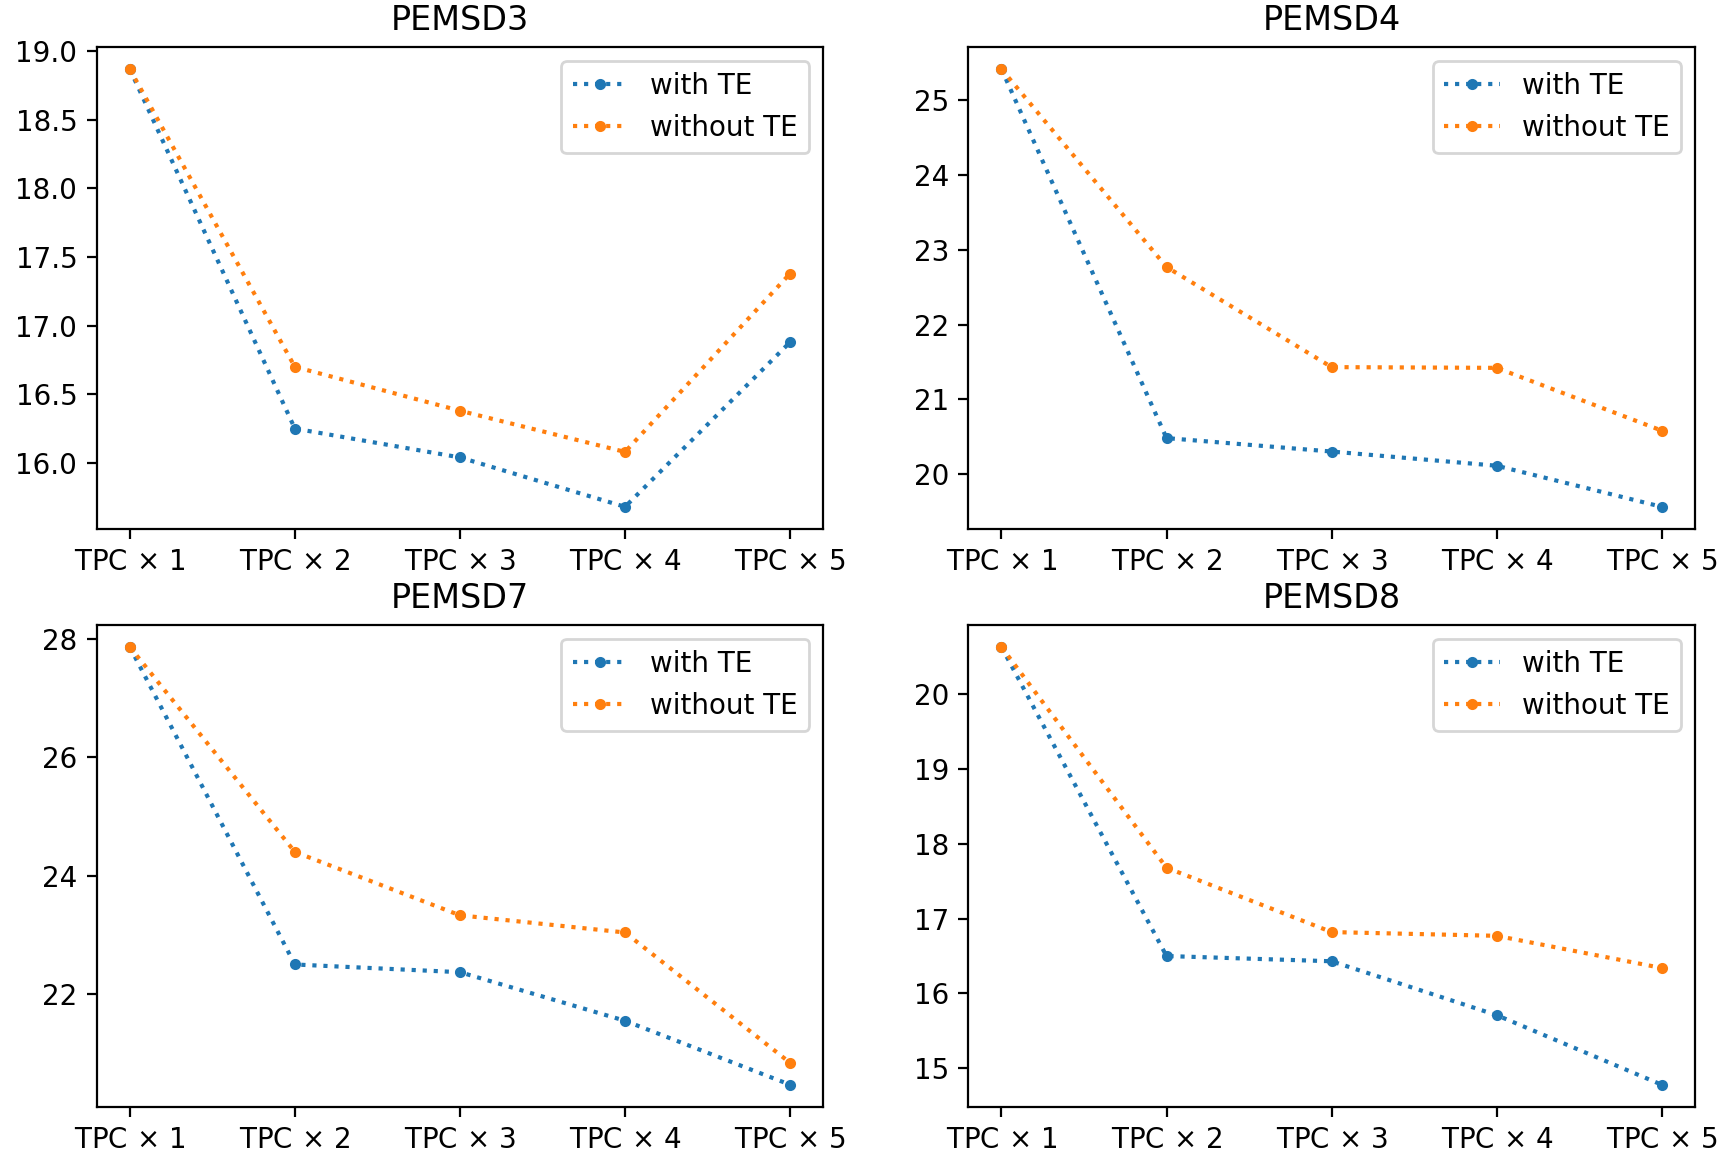
\includegraphics[width=0.48\textwidth]{pictures/Ablation.png}
    \caption{The MAE sensitivity to different settings of MS-GAT on PEMSD3, PEMSD4, PEMSD7 and PEMSD8.}
    \label{fig:ablation}
\end{figure}

First, the multi-component structure is shown effective for spatio-temporal forecasting. Importantly, adding more components (\textit{TPCs})  to MS-GAT can contribute to accurate prediction. However, it does not mean  more components lead to the better results. As shown in Table~\ref{tab:ablation}, the model setting with four \textit{TPCs} achieves the best performance on PEMSD3, while the prediction on PEMSD4, PEMSD7 and PEMSD8 requires five \textit{TPCs} for the best. This is owing to that the traffic conditions of different physical road networks show specific spatio-temporal system complexities. When taking more historical horizons as the input of each \textit{TPC} separately, the prediction of MS-GAT would worsen instead. In other words, more input sequences to model could be harmful or meaningless. Therefore, the number of \textit{TPC} components is an important hyperparameter, which determines the performance of MS-GAT.

Second, the \textit{TE} is proven very necessary for ensuring the model accuracy. The  results in Table~\ref{tab:ablation} show the model settings with \textit{TE} are consistently superior to those without \textit{TE}. It demonstrates the traffic conditions at the past distinct time horizons have different correlation strengths with the one at the same future time horizon. Thus, the prediction effect can be significantly improved through deploying \textit{TE} in MS-GAT.

Third, the channel relation is confirmed essential for modeling the dynamics of traffic systems. The results exhibited in the last column of Table~\ref{tab:ablation} draw from the case of skipping over the channel relation when MS-GAT is under its best model setting (i.e., the one that produces the bold number in each row of Table~\ref{tab:ablation}). Clearly, when those potential channel relations coupled among traffic signals are not taken care of, the performances of MS-GAT degrade significantly. The experimental results also substantiate the effectiveness of \textit{CAttention} that applies attention mechanism to capture the channel relation of traffic signals. As a result, focusing on more interactive relations coupled within complex traffic systems contributes to improving the capability of predictive model.

\subsection{Case study}

\begin{figure}[!ht]
    \centering
    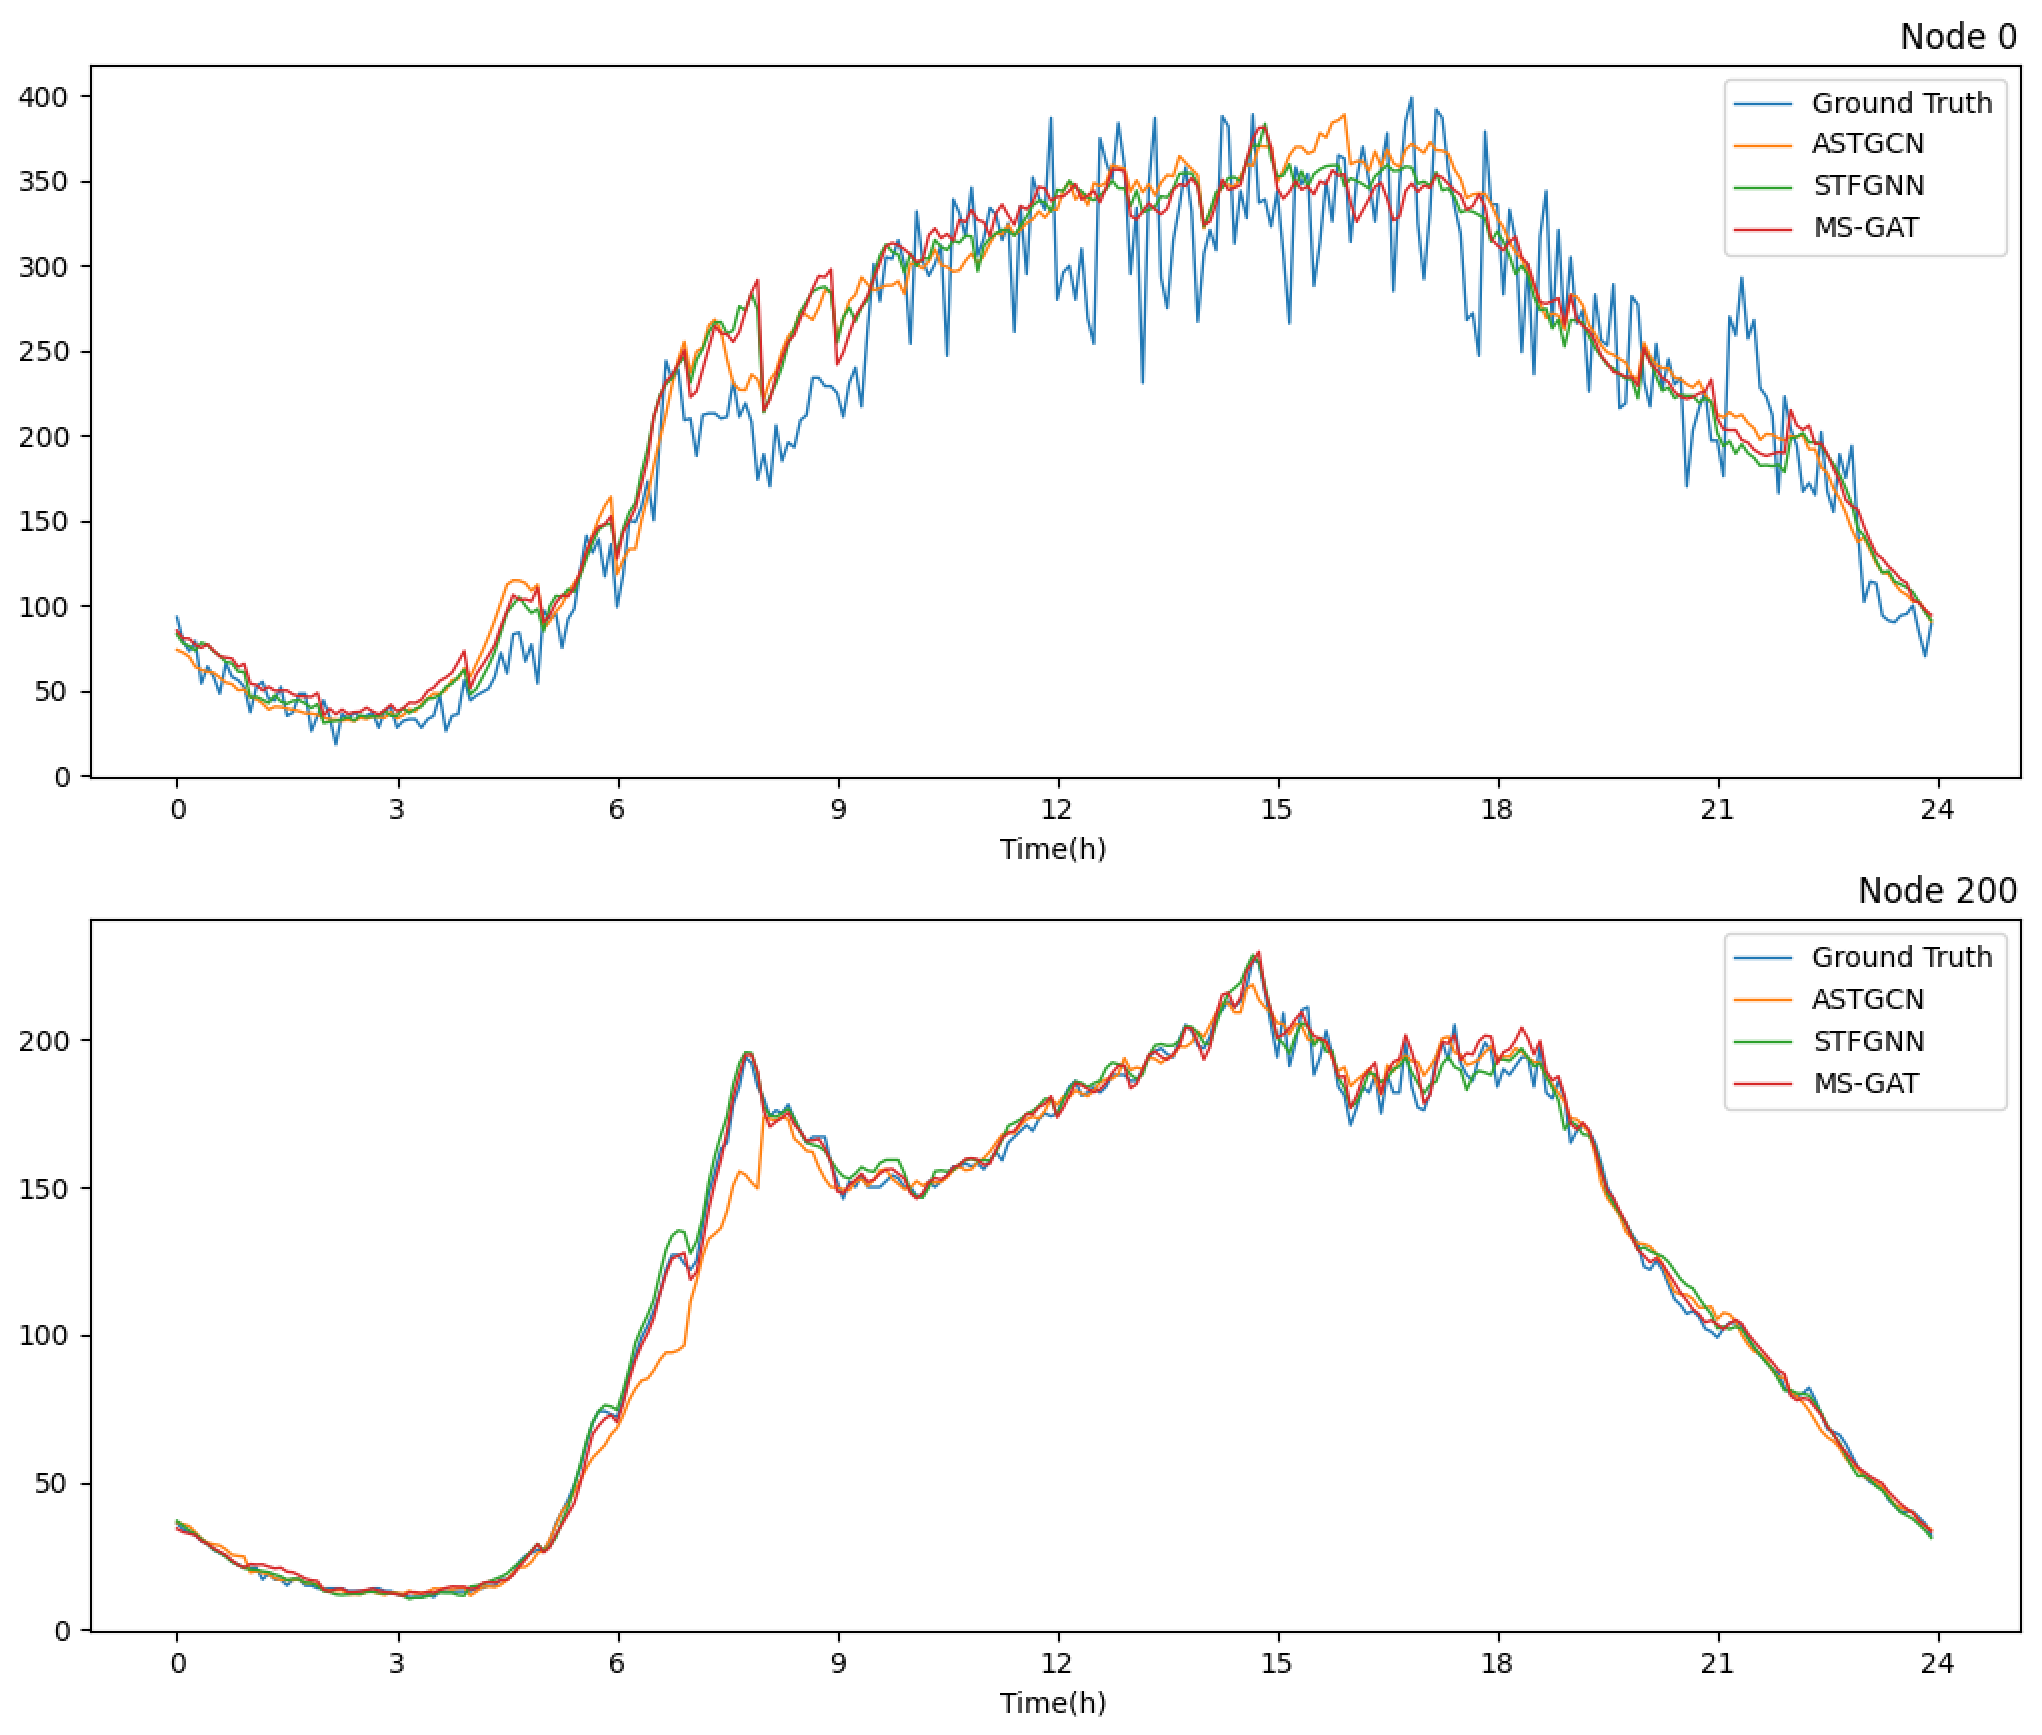
\includegraphics[width=0.48\textwidth]{pictures/Case_1.png}
    \caption{A case study of the traffic flow prediction at Node 0 and Node 200.}
    \label{fig:case_1}
\end{figure}

\begin{figure}[!ht]
    \centering
    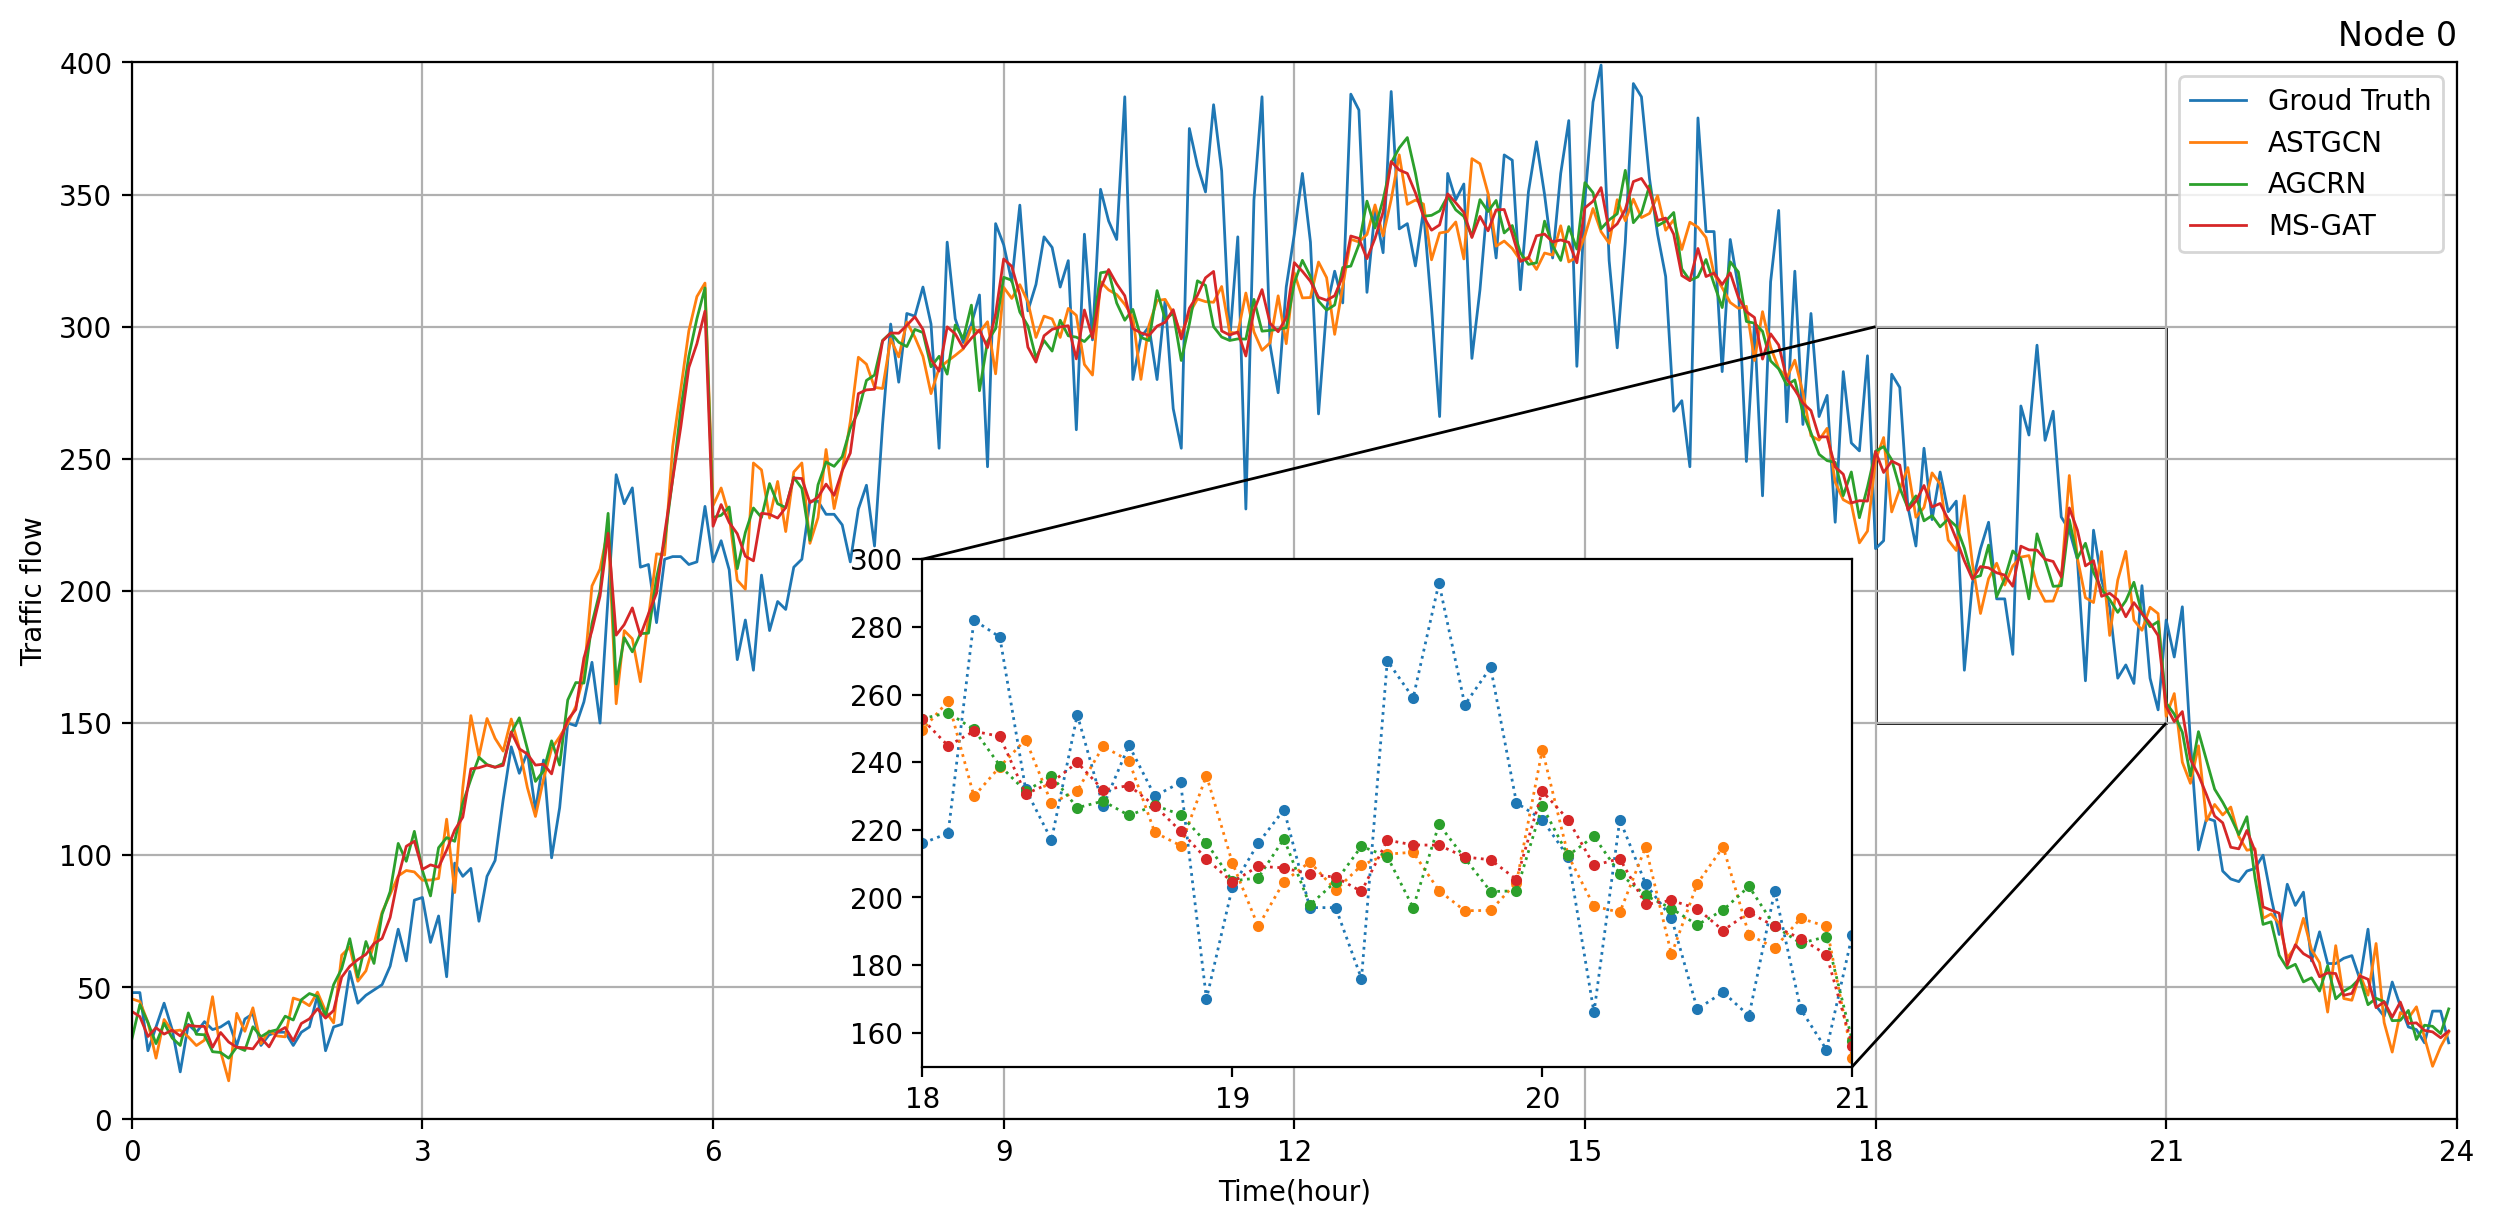
\includegraphics[width=0.48\textwidth]{pictures/Case_2.png}
    \caption{Illustration of the prediction error at Node 0.}
    \label{fig:case_2}
\end{figure}

To further investigate the performance of MS-GAT, we also conduct a case study to intuitively show its prediction effect. We select two traffic nodes Node 0 and Node 200 in PEMSD4 and plot their future 24-hour traffic flow prediction results separately in Fig.~\ref{fig:case_1} to compare two state-of-the-art models ASTGCN and AGCRN against our proposed MS-GAT to carry out every 1-hour interval forecasting. It can be observed that, compared to those competitive models, the prediction curves of MS-GAT on both Node 0 and Node 200 are better aligned to the temporal trends of their ground-truth traffic conditions. Fig.~\ref{fig:case_1} shows that the prediction error at Node 0 is significantly higher than that at Node 200. This is because there exist some frequent uncertain interference factors or random traffic events at Node 0 which induce the abrupt changes of traffic flow, thus exhibiting a kind of short-term recurrent blocked-unblocked traffic condition that is very challenging to be accurately estimated in practice. Fig.~\ref{fig:case_2} further shows that MS-GAT is slightly superior to the other two models, indicating that MS-GAT could adapt to such  abrupt changes of traffic conditions by its distinctive model design and parameter learning. Therefore, when performing the traffic flow prediction on the whole road network consisting of various geospatial nodes, the RMSE improvement of MS-GAT is not as significant as that in terms of MAE, which is consistent with our prior experimental results presented in Table~\ref{tab:pemsd3-8}. The reason for that is the physical road network in PEMSD4 contains many traffic nodes with short-term recurrent blocked-unblocked traffic condition like Node 0. This also triggers a future direction, i.e., further improving the stability and robustness of traffic prediction models by exploring the influence of the sharp changes of traffic conditions over nodes.



\section{Discussion}
Machine learning technique motivates the development of the ITS community in recent years. In particular, many deep-learning-based models including the aforementioned modern neural networks are successively proposed to meet the challenging traffic prediction task. The design and formulation of these impressive predictive models usually relies on some assumptions or specific observations on the recorded traffic signal data, and thus forming diverse network architectures of such learning models in terms of their respective inductive biases. Specifically, early deep-learning-based efforts started with treating traffic prediction as a sequence learning issue. They further naturally employed canonical RNNs (e.g., LSTM) to build the roughly similar backbone of their deep neural network architectures. The backbone models the dynamics of traffic system by focusing on the temporal dependencies hidden inside traffic conditions. After that, other studies also paid attention to the influence of potential spatial dependencies among traffic conditions on dynamic traffic system. They successively exploited well-established CNNs or emerging GNNs to enrich the above backbone for elaborating their distinctive model architectures. These models (e.g., the above baseline methods) all deliver excellent results, and thus a unified framework, called Spatial-Temporal Graph Neural Networks (STGNNs) \cite{2019A}, is formed for modeling dynamic traffic systems based on the pioneering works.

We argue that, like other complex systems, a traffic system is a coupled traffic network consisting of various channels and nodes, where traffic signals interact and are coupled with each other. Specifically, the dynamics of traffic conditions are associated with a variety of traffic signals and external environment (such as weather data), which interact and are coupled with each other as well. By viewing a traffic system as a coupled traffic network with multi-sensor traffic signals interacting and coupled, we can further model couplings in multi-modal traffic data and external data. We notice that the current widely-adopted framework STGNNs implies its inductive bias of modeling traffic systems likewise. Those models following the framework prefer to merely focus on two kinds of acquainted dependency relations (i.e., spatial and temporal relations) coupled inside traffic conditions. And they use an alternating neural network forward computation manner to pick up the two relations in turn, so as to excavate their coupling relations (i.e., so-called spatio-temporal relations) indirectly. Compared with them, MS-GAT attempts to improve the model bias by (1) shedding light on another noteworthy dependency relations (i.e., channel relations) that are also coupled inside traffic conditions, and (2) conceiving a synchronous neural network forward computation manner to separately identify all possible dependency relations of concern to us and explicitly assess their coupling strengths with each other to predictions. Ultimately, the above experimental results have also verified the superiority of our inductive bias to modeling dynamic traffic conditions. 

Furthermore, we notice that a burgeoning neural network architecture, called Transformer \cite{vaswani2017attention}, has flourished in the field of nature language processing (NLP) in the past few years. This architecture different from CNNs, RNNs and GNNs, can provide the relationships between features of different input data via the attention mechanism. Its power in sequence learning issue inspires other communities (e.g., computer vision, CV) to investigate the use of Transformer for their specific tasks. Not surprisingly, the novel architecture has also attracted a few ITS researchers to explore its potential in traffic predictions. The most recent ASTGNN \cite{2021Learning} is such a impressive transformer-like predictive model. It leverages Transformer to conduct the forward computation of the STGNNs framework for long-term prediction, and elaborates its distinctive inductive bias to concretize the transformer-based encoder-decoder framework with valuable considerations (e.g., explicitly modeling the periodicity and spatial heterogeneity). 

By experimental comparisons on the PEMSD4 dataset, ASTGNN performs slightly better than MS-GAT on the metrics of MAE, MAPE and RMSE by 5.6\%, 7.9\% and 2.1\% respectively for the next 1-hour prediction task. Definitely, the transformer-based architecture of ASTGNN has played a great role for the learning ability of the transformer-like model to make long-term predictions. It is because that massive multi-head attentions in Transformer with global receptive fields as well as unique embedding mechanisms of relevant information can effectively assist those transformer-based models to excavate more significant features for the sequence-to-sequence task. Meanwhile, ASTGNN also reveals its own inductive bias of modeling the dynamics of traffic conditions across both spatial and temporal dimensions. Concretely, except for taking the transformer-like framework as its backbone, ASTGNN also deliberately devises two important modules: (1) a trend-aware self-attention module that enables the self-attention being aware of the local temporal context, and (2) a dynamic graph convolution module that models the spatial dependencies. Notwithstanding, in contrast to MS-GAT, this kind of transformer-like predictive model also faces extra challenges, including: (1) \textit{huge amount of calculation}. Due to complex learning mechanisms and overparametered networks in Transformer, those transformer-like predictive models are typically difficult to train. They depend on a huge number of training data. For instance, on our above experimental setting with 2080TI, ASTGNN need to cost around 220s to conduct an epoch of training, while MS-GAT just costs about 100s for every epoch; (2) \textit{insufficiency of parallel capability}. The transformer-like predictive models like ASTGNN are all equipped with a heavy decoder that performs in an auto-regressive manner. It means that every output sequence of their decoders is generated one by one. Namely, the current prediction relies on the previous result. Instead, the decoding process of MS-GAT is developed to be a simple regressor based on neural network, which produces output sequences in a one-step manner. Its encoding process is designed to be a structure with multiple independent branches, where each branch is responsible for identifying a specific dependency relation coupled inside traffic conditions (e.g., spatial, temporal or channel relations). Importantly, each branch can be conveniently deployed on a separate computation resource (e.g., CPU or GPU) for achieving parallel acceleration. 

To sum up, owing to its own architectural characteristics, MS-GAT is more applicable for short-term traffic prediction, and also suitable for the case of deploying parallel settings for pursuing real-time effect. Moreover, 

inspirited by the newly proposed 

ASTGNN that paves the way for transferring the success of pure transformer model in NLP to the traffic prediction task in ITS, we are also thinking about applying Transformer to MS-GAT, e.g., attaching a transformer-based decoder in MS-GAT for more accurate long-term prediction. 

\section{Conclusions}
Despite of the great success of prior works, traffic prediction is still a challenging task in ITS. By viewing a traffic system as a coupled traffic network, in this paper, we focus on the continuous signals from various channels and nodes interacting and coupling with each other in terms of temporal, spatial and spatio-temporal aspects of traffic conditions. The multi-aspect traffic signal couplings are modeled by a deep graph network MS-GAT, which characterizes multi-dimensional, time-evolving and multi-relational traffic interactions in the road network. Concretely, MS-GAT explicitly models the latent relations between diversified traffic signals in terms of \textit{channel relations} and integrates them  with \textit{spatial} and \textit{temporal relations} in a synchronous way into the neural traffic graph for forecasting. These are modeled by (1) a module MEAM stacking replicas of deep learning architectures to capture the complicated spatio-temporal dynamics of traffic conditions and their multi-relations and influence on future traffic conditions, and (2) a multi-component structure TPCs that adopts a time gated fusion mechanism to adaptively focus on the traffic conditions at different past stages. Further, MS-GAT maintains a small number of parameters with a convenient multi-dimensional self-attention scheme applicable to any data with multi-dimensional features. We substantially test MS-GAT on five real-world datasets against six state-of-the-art graph neural networks for traffic prediction, which show that MS-GAT outperforms the baselines. 

MS-GAT is a general spatio-temporal forecasting framework, applicable to other spatio-temporal structured sequence forecasting scenarios, such as preference prediction in recommender systems and air quality forecasting, since it is characterized by providing a multi-view representation for each node in graphs and a multi-relational representation for graph-based complex systems. In ITS, in the case of the data from different traffic modes (e.g., bus, private car, bike) or external modes (e.g., passengers or weather) in an identical traffic region is available, MS-GAT can also attempt to handle these multi-modal data and their interactions through treating each modal data as a separate information channel to manipulate. We argue that there exist some potential causal associations between those available multi-modal data and expectations in traffic prediction tasks, such as the impact of current rainfall on future traffic flow in a road network, whereas MS-GAT just can deal with that. 

Besides, MS-GAT can be also expanded in the following directions. First, we will further optimize the network structure and parameters to improve the prediction accuracy on sharp changes of traffic conditions that may be induced by external factors, e.g., weather or abnormal events. Second, like other spatio-temporal forecasting methods, we will also explore the mechanism of modeling the spatio-temporal dependencies for evolving graph structures.

\bibliographystyle{IEEEtran}
\bibliography{IEEEabrv, references}

\begin{IEEEbiography}[{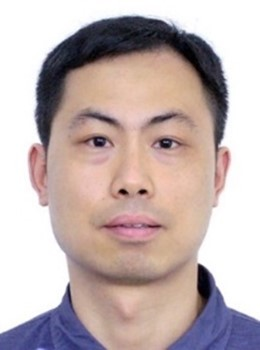
\includegraphics[width=1in,height=1.25in,clip,keepaspectratio]{pictures/Huang.jpg}}]{Jing Huang} received Ph.D. in computer science from Huazhong University of Science and Technology, China in 2006. Before joining Wuhan University of Technology as an Associate Professor, he worked in Huazhong University of Science and Technology as a post-doctoral fellow. He visited University of Technology Sydney as a visiting scholar between August 2015 and August 2016. His research interests include but not limited to machine learning, data mining, intelligent transportation systems, pattern recognition and computer vision.
\end{IEEEbiography}

\begin{IEEEbiography}[{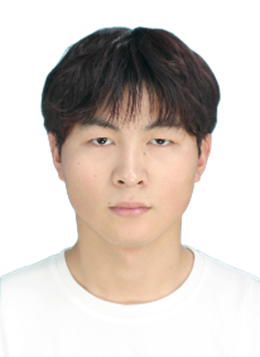
\includegraphics[width=1in,height=1.25in,clip,keepaspectratio]{pictures/Luo.png}}]{Kun Luo} received his B.S. degree in logistics engineering from Wuhan University of Technology, Wuhan, China in 2020. He was a postgraduate in the school of computer science and technology, Wuhan University of Technology, China when this work was done. His research interests include machine learning and pattern recognition in intelligent transportation systems (ITS).
\end{IEEEbiography}

\begin{IEEEbiography}[{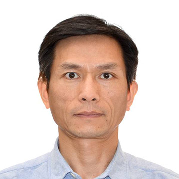
\includegraphics[width=1in,height=1.25in,clip,keepaspectratio]{pictures/Cao.pdf}}]{Longbing Cao}(SM'06) received a PhD degree in pattern recognition and intelligent systems and another PhD in computing sciences. He is a Professor at the University of Technology Sydney and an Australian Research Council Future Fellow (professorial level). His current research interests include data science, data mining, machine learning, behavior informatics, artificial intelligence and intelligent systems, and their enterprise applications.
\end{IEEEbiography}

\begin{IEEEbiography}[{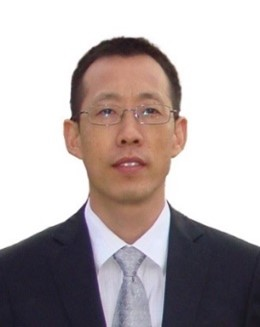
\includegraphics[width=1in,height=1.25in,clip,keepaspectratio]{pictures/Wen.jpg}}]{Yuanqiao Wen} received Ph.D. in computer science from Huazhong University of Science and Technology, China in 2006. He is currently a Professor and Ph.D. supervisor in the National Engineering Research Center for Water Transport Safety, Wuhan University of Technology, China. He visited Technische Universiteit Delft as a senior visiting scholar between November 2016 and December 2016. Dr. Wen’s research interests mainly include but not limited to intelligent transportation systems, data mining, artificial intelligence, and transport safety.
\end{IEEEbiography}

\begin{IEEEbiography}[{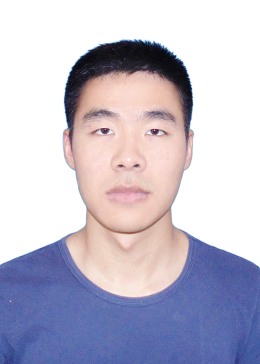
\includegraphics[width=1in,height=1.25in,clip,keepaspectratio]{pictures/Zhong.png}}]{Shuyuan Zhong} received his B.S. degree in computer science from Wuhan University of Technology, Wuhan, China, in 2019. He was a postgraduate in the school of computer science and technology, Wuhan University of Technology, China when this work was done. His research interests include deep learning and graph neural networks.
\end{IEEEbiography}

\end{document}